\documentclass[12pt, letterpaper, preprint, comicneue]{aastex63}
%\usepackage[default]{comicneue} % comic sans font for editing
\usepackage[T1]{fontenc}
%%% This file is generated by the Makefile.
\newcommand{\giturl}{\url{https://github.com/IQcollaboratory/galpopFM}}
\newcommand{\githash}{16d38a2}\newcommand{\gitdate}{2021-01-25}\newcommand{\gitauthor}{ChangHoon Hahn}

\usepackage{color}
\usepackage{amsmath}
\usepackage{natbib}
\usepackage{ctable}
\usepackage{bm}
\usepackage[normalem]{ulem} % Added by MS for \sout -> not required for final version
\usepackage{xspace}
\usepackage{csvsimple} 

\usepackage{graphicx}
\usepackage{pgfkeys, pgfsys, pgfcalendar}


% typesetting shih
\linespread{1.08} % close to 10/13 spacing
\setlength{\parindent}{1.08\baselineskip} % Bringhurst
\setlength{\parskip}{0ex}
\let\oldbibliography\thebibliography % killin' me.
\renewcommand{\thebibliography}[1]{%
  \oldbibliography{#1}%
  \setlength{\itemsep}{0pt}%
  \setlength{\parsep}{0pt}%
  \setlength{\parskip}{0pt}%
  \setlength{\bibsep}{0ex}
  \raggedright
}
\setlength{\footnotesep}{0ex} % seriously?

% citation alias

% math shih
\newcommand{\setof}[1]{\left\{{#1}\right\}}
\newcommand{\given}{\,|\,}
\newcommand{\lss}{{\small{LSS}}\xspace}

\newcommand{\Om}{\Omega_{\rm m}} 
\newcommand{\Ob}{\Omega_{\rm b}} 
\newcommand{\OL}{\Omega_\Lambda}
\newcommand{\smnu}{M_\nu}
\newcommand{\sig}{\sigma_8} 
\newcommand{\mmin}{M_{\rm min}}
\newcommand{\BOk}{\widehat{B}_0} 
\newcommand{\hmpc}{\,h/\mathrm{Mpc}}
\newcommand{\bfi}[1]{\textbf{\textit{#1}}}
\newcommand{\parti}[1]{\frac{\partial #1}{\partial \theta_i}}
\newcommand{\partj}[1]{\frac{\partial #1}{\partial \theta_j}}
\newcommand{\mpc}{{\rm Mpc}}
\newcommand{\eg}{\emph{e.g.}}
\newcommand{\ie}{\emph{i.e.}}

\let\oldAA\AA
\renewcommand{\AA}{\text{\normalfont\oldAA}}
% cmds for this paper 
\newcommand{\gr}{g{-}r}
\newcommand{\fnuv}{FUV{-}NUV}
\newcommand{\sfr}{{\rm SFR}}
\newcommand{\ssfr}{{\rm SSFR}}
\newcommand{\mtaum}{m_{\tau,M_*}}
\newcommand{\mtaus}{m_{\tau,{\rm SSFR}}}
\newcommand{\ctau}{c_\tau}
\newcommand{\mdeltam}{m_{\delta,M_*}}
\newcommand{\mdeltas}{m_{\delta,{\rm SFR}}}
\newcommand{\cdelta}{c_\delta}
\newcommand{\eda}{EDA}


\newcommand{\specialcell}[2][c]{%
  \begin{tabular}[#1]{@{}c@{}}#2\end{tabular}}
% text shih
\newcommand{\foreign}[1]{\textsl{#1}}
\newcommand{\etal}{\foreign{et~al.}}
\newcommand{\opcit}{\foreign{Op.~cit.}}
\newcommand{\documentname}{\textsl{Article}}
\newcommand{\equationname}{equation}
\newcommand{\bitem}{\begin{itemize}}
\newcommand{\eitem}{\end{itemize}}
\newcommand{\beq}{\begin{equation}}
\newcommand{\eeq}{\end{equation}}

%% collaborating
\newcommand{\todo}[1]{\marginpar{\color{red}TODO}{\color{red}#1}}
\definecolor{orange}{rgb}{1,0.5,0}
\newcommand{\ch}[1]{{\color{orange}#1}}
\newcommand{\chedit}[1]{{\color{orange}#1}}
\newcommand{\tks}[1]{{\color{blue}{\bf TKS:} #1}}
\newcommand{\tksedit}[1]{{\color{blue}#1}}

\begin{document} \sloppy\sloppypar\frenchspacing 

\title{IQ Collaboratory III Empirical Dust Attenuation Models: Taking Hydrodynamical Simulatons with a Grain of Dust}
\date{\texttt{DRAFT~---~\githash~---~\gitdate~---~NOT READY FOR DISTRIBUTION}}

\newcounter{affilcounter}
\author{ChangHoon Hahn}
\altaffiliation{hahn.changhoon@gmail.com}
\affil{Department of Astrophysical Sciences, Princeton University, Peyton Hall, Princeton NJ 08544, USA} 
%\affil{Lawrence Berkeley National Laboratory, 1 Cyclotron Rd, Berkeley CA 94720, USA}
%\affil{Berkeley Center for Cosmological Physics, University of California, Berkeley CA 94720, USA}

\author{Tjitske K. Starkenburg}
\affil{Center for Interdisciplinary Exploration and Research in Astrophysics (CIERA) and \\Department of Physics and Astronomy, 1800 Sherman Ave, Evanston IL 60201, USA}

\author{IQ Collaboratory}

\begin{abstract}
    We present the Empirical Dust Attenuation (\eda) framework for applying
    dust attenuation to galaxy formation models.
    \ch{
        The \eda~provides a flexible prescription for assigning realistic dust
        attenuation to simulated galaxies based on their physical properties
        ($M_*$, $\ssfr$) and the \cite{noll2009} attenuation curve. 
    }
    We apply the \eda~separately to three state-of-the-art cosmological
    hydrodynamical simulations (SIMBA, IllustrisTNG, and EAGLE) and forward
    model their optical and UV
    color-magnitude relations, $(\gr) - M_r$ and $(\fnuv)-M_r$. 
    We then compare the simulations to a $M_r < -20$ complete SDSS galaxy sample
    using likelihood-free inference. 
    \ch{
        We find that dust attenuation is necessary for any of the simulations
        to match the observations. 
    }
    With the \eda, we accurately reproduce the color-magnitude relations of the
    observational sample for TNG and EAGLE. 
    For SIMBA, we struggle to reproduce observations due to an overprediction
    of starburst galaxies. 
    \ch{ 
        Examining the attenuation curves predicted by the \eda~for TNG and
        EAGLE, we find good agreement with the observed attenuation--slope
        relations and attenuation curve of star-forming galaxies.
    }
    Beyond reproducing observations,
    the \eda~also sheds light on dust attenuation in quiescent galaxies, which
    is challenging to measure observationally. We find that quiescent galaxies 
    have significant UV and optical attenuation but with much shallower
    slopes than star-forming galaxies. 
    \ch{ 
        Overall, we find that more massive galaxies in the simulations require
        higher dust attenuation, 
    }
    while galaxies with higher specific star formation rates have steeper 
    attenuation curves.
    In addition to improving our understanding of dust in galaxies, our results
    underscore the advantages of the \eda~and the forward modeling approach. 
\end{abstract}

\keywords{
keyword1 -- keyword2 -- keyword3
}

% --- intro ---  
\section{Introduction} \label{sec:intro} 
Dust in the interstellar medium of a galaxy can dramatically impact the
observed light from the galaxy over the full range of the electromagnetic spectrum. 
It emits in the infrared (IR) and modifies the galaxy's stellar radiation
through absorption and scatter from the near-infrared (NIR) to ultraviolet
(UV). Dust can, therefore, dramatically impact the physical properties of
galaxies we infer from optical and UV light, such as star
formation rate ($\sfr$), stellar mass ($M_*$), or stellar ages~\citep[see
reviews by][]{walcher2011, conroy2013}. Since these properties are the
building blocks for our understanding of galaxies and how they evolve,
a better understanding of dust not only provides insights into the physical
processes related to dust, but it also underpins all galaxy studies.  

The combined effect of dust on the spectral energy distribution (SED) of a
galaxy is typically described using an attenuation curve, $A(\lambda)$.
Observations have now established the major features in $A(\lambda)$. In the UV, the 
curve steeply rises due to absorptions by small grains. At $2175\AA$, in the 
near-UV (NUV), there is absorption bump referred to as the ``UV dust bump''. 
At longer wavelengths, the curves on take a power-law shape. For an overview, we 
refer to reviews by \cite{calzetti2001, draine2003, galliano2018}. Attenuation
curves, however, are not universal. Observations find a wide range of
attenuation curves in the local Universe~\citep{wild2011, battisti2017,
salim2018, salim2020} as well as at high redshifts~\citep[\eg][]{reddy2015,
salmon2016}.

% summarize studies that looked at the connection between attenuation curves
% and galaxy properties (wild2011 battisti2016, battisti2017, and
% salim2018). List the hodge-podge correlations. Talk about how Salim claims
% that the attenuation-slope relations account for everything, but there's no
% clear concensus. Restate the importance of understanding the attenuaion
% curves properly.
To understand the origin of this variation in attenuation curves, a number of
observational  works have examined the correlation between dust attenuation and
galaxy properties. Using 23,000 star-forming galaxies in the Sloan Digital
Sky Survey (SDSS), \cite{wild2011} found that the slope of the attenuation
curves varies strongly with galaxy axial ratio and weakly with specific SFR (SSFR).
Similarly, \cite{battisti2017}, from 5,500 star-forming galaxies, found tentative
trends with stellar age, specific star formation rate, stellar mass, and
metallicity. Meanwhile, \cite{salim2018}, from 230,000 galaxies in the
GALEX-SDSS-WISE Legacy Catalog 2 (GSWLC2), find a significant $M_*$ 
dependence on the slope. They argue that this is caused by the underlying 
``attenuation-slope relation'', a trend between the amplitude of the 
$V$-band attenuation ($A_V$) and slope, where galaxies with higher $A_V$ have
shallower slopes.
At low attenuation, dust scattering dominates absorption so the 
attenuation curve steepens because red light scatters isotropically while blue light
scatters forward~\citep{gordon1994, witt2000, draine2003}. %, which causes more optical-to-IR light to escape the galaxy than UV light
At high attenuation dust absorption is dominant and the attenuation curve is
shallower~\citep{chevallard2013}. 
Nevertheless, there is still no clear consensus on the
connection between attenuation curves and galaxy properties. Also, studies 
so far have focused on star-forming galaxies and little is known
about dust attenuation in quiescent galaxies. 

%Assumptions on the attenuation curve can dramatically impact the physical properties inferred from fitting the SED~\citep[\eg][]{kriek2013, shivaei2015, reddy2015, salim2020}. Moreover, the more we understand about dust the more constraining power we can keep for 
Alongside observations, theoretical efforts that model radiative transfer of
stellar light through a dusty ISM also provide insights into dust attenuation.
Radiative transfer models span a wide range of geometric configurations of
stars and dust. For instance, models focused on isolating the physical effects
of dust have considered simple slab or shell-like dust geometries illuminated
by stellar radiation~\citep[\eg][]{witt1996, witt2000, seon2016}. Other models,
focused on modeling dust attenuation in galaxies as a whole, have applied 3D
dust radiative transfer in hydrodynamic simulations of idealized
galaxies~\citep[\eg][]{jonsson2006, rocha2008, hayward2015, natale2015,
hou2017}. Dust attenuation has also been examined in a cosmological context
using semi-analytic models (SAMs) that do not track baryonic growth directly 
but make simple physically motivated assumptions about the resulting galaxy
properties from dark matter growth~\citep[\eg][]{granato2000,
fontanot2009, wilkins2012, gonzalez-perez2013, popping2017}. Lastly, radiative transfer
models have recently been applied to cosmological hydrodynamical
simulations~\cite[\eg][]{camps2015, narayanan2018, trayford2020}. As in
observations, simulations find significant variation in attenuation
curves. %They also reproduce the shape of the attenuation-slope relation. 

% Why can't we use RT for everything. 
Despite their progress, there are still major challenges for radiative
transfer models. For instance, they produce attenuation-slope relations that
are significantly steeper than observations. Many models also require
significant hand-tuning (\eg~propagating rays/photons into
particular cells). Assumptions in the underlying dust grain models also produce
systematic uncertainties that are difficult to quanitfy~\citep[see][for a
review]{steinacker2013}. Lastly, radiative transfer models 
are computationally expensive. Applying a range of radiative transfer dust
models to multiple simulations for comparisons is prohibitive. Using Markov
Chain Monte Carlo to sample them for parameter exploration or to marginalize
over the impact of dust would be {\em intractable}. 

%motivation for an empirical dust attenuation model
In this paper, we take a different approach and present the Empirical Dust
Attenuation (\eda) model, a flexible framework for statistically applying dust
attenuation to galaxy populations. The \eda~model assigns, to every galaxy, a
different dust attenuation curve. We present attenuation curves that are parameterized with
a functional-form used in observational studies~\citep{noll2009} and the
parameters of the curve for each galaxy (\eg~optical depth, slope) are sampled
from distributions set by the \eda~model parameters and the galaxy's properties.  
By sampling the attenuation curve parameters, it produces realistic variations 
among the attenuation curves. The \eda~does not seek to produce realistic dust 
attenuation for individual galaxies, like radiative transfer models. Instead, 
it aims to produce realistic dust attenuations for a large ensemble of galaxies
that enables direct comparison across galaxy populations. 

There are a number of advantages to our \eda~approach. The \eda~uses the same
functional-form for the attenuation curves as observational studies, so
predictions of the model can easily be compared to observational constraints. 
We also formulate the \eda~parameters so that they are easily interpretable and
directly reveal correlations between dust attenuation and galaxy properties.
Lastly, the \eda~model is computationally inexpensive. 

The \eda~model, with its flexibility and speed, provides a crucial step in a
{\em forward modeling approach} to comparing simulations to
observations~\citep[\eg][]{nelson2018, baes2019, trcka2020, dickey2020}.
In the standard approach, the galaxy properties (\eg~SFR, $M_*$) predicted by
simulations are compared to those derived from observations. In the forward
modeling approach, observable quantities (\eg~magnitude, color) are {\em forward
modeled} for each galaxy in the simulations; then the simulations are compared 
to observations in observational space. With a forward modeling approach, 
comparisons are not limited by variations, inconsistencies, and biases of different
observational methods for measuring galaxy properties (\eg~different tracers of
SFR or $M_*$). Selection functions and systematic effects can also be accounted
for in the forward model. 

Of course, to produce realistic observables of simulated galaxies, the forward
model must include some prescription for applying dust attenuation. In
principle, a radiative transfer model can be used for this purpose; however,
its computational cost would severely limit any exploration of the ``dust
parameters''. With the \eda, however, we can apply a wide range of realistic
dust attenuation to simulated galaxies in a matter of seconds and easily
explore and sample the \eda~parameter space to infer the 
relationship between dust attenuation and galaxy properties. {\em For readers 
uninterested in dust}, the \eda~provides a way to treat dust parameters as
{\em nuisance} parameters and tractably marginalize over dust attenuation. 

In this work, we present a simple \eda~model that uses the \cite{noll2009}
attenuation curve parameterization and includes correlations between dust
attenuation and galaxy $M_*$ and $\sfr$ (Section~\ref{sec:dem}). We apply 
the \eda~separately to three state-of-the-art cosmological large-scale hydrodynamical 
simulations (SIMBA, IllustrisTNG, and EAGLE), which we describe in
Section~\ref{sec:sims}, and compare them to a volume-limited galaxy sample from SDSS
and GALEX observations (Section~\ref{sec:obs}). In Section~\ref{sec:dem}, we
describe our \eda~model in detail. Finally, in Section~\ref{sec:results}, we
present the results of our comparison and discuss their implications for our
understanding of dust attenuation as well as of its connection to galaxy properties. 

% --- data ---  
\section{Data}\label{sec:sims}
\begin{figure}
\begin{center}
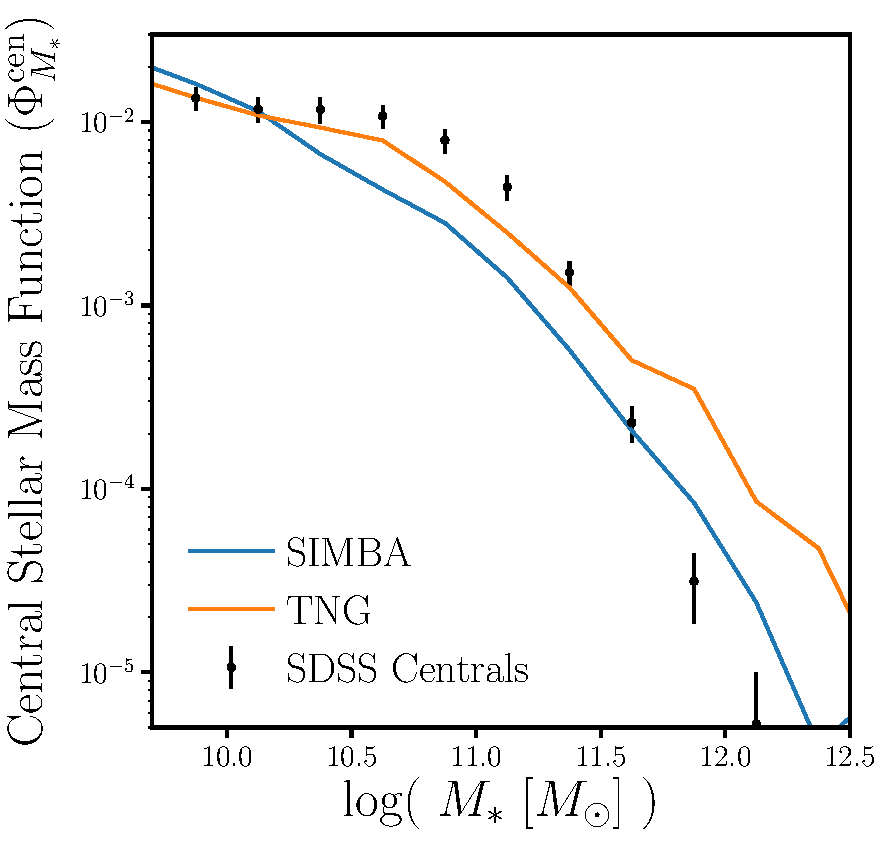
\includegraphics[width=0.5\textwidth]{figs/smfs.pdf} 
    \caption{The stellar mass functions of central galaxies, $\Phi^{\rm
    cen}_{M_*}$, of the SIMBA (orange) and TNG (blue) simulations compared to
    the SDSS $\Phi^{\rm cen}_{M_*}$. The uncertainties for the SDSS $\Phi^{\rm
    cen}_{M_*}$ are derived using jackknife resampling and SDSS centrals are
    identified using a halo-based group finder (Section~\ref{sec:obs}). For
    SIMBA and TNG galaxies, we calculate $M_*$ as the total stellar mass within
    the host halo, excluding contributions from any subhalos; centrals are
    classified based on their individual definition (Section~\ref{sec:tng}
    and~\ref{sec:simba}). {\color{red} should we include total SMF...?} 
    {\em The simulations and observations have loosely consistent $\Phi^{\rm
    cen}_{M_*}$.} 
    }
\label{fig:smf}
\end{center}
\end{figure}

\subsection{SDSS DR7 Central Galaxies} \label{sec:obs} 
Throughout the paper we compare the simulations and models described below
to the observed SDSS central galaxy sample from the \cite{tinker2011} group
catalog. The group catalog, first, selects volume-limited sample of galaxies at
$z \approx 0.04$ with $M_r < -18$ and complete above $M_* > 10^{9.4}
h^{-2}M_\odot$ from the NYU Value-Added Galaxy
Catalog~\citep[VAGC;][]{blanton2005} of SDSS DR7~\citep{abazajian2009}. The
stellar masses are estimated using the $\mathtt{kcorrect}$
code~\citep{blanton2007a} assuming a~\cite{chabrier2003} initial mass
function. 

Central galaxies are then identified using a halo-based group finder that uses
the abundance matching ansatz to iteratively  assign halo masses to groups.
Every group contains one central galaxy, which by definition is the most
massive, and a group can contain $\ge0$ satellites. As with any group finder,
galaxies are misassigned due to projection effects and redshift space
distortions; however, the central galaxy sample has a purity of ${\sim}90\%$
and completeness of ${\sim}95\%$~\citep{tinker2018}. 

\subsection{Illustris TNG} \label{sec:tng}
\todo{describe what galaxy properties (SFH, ZH, etc) are available} 

\subsection{SIMBA} \label{sec:simba}
\todo{describe what galaxy properties (SFH, ZH, etc) are available} 

In Figure~\ref{fig:smf}, we compare the stellar mass function (SMF) of our SDSS
central galaxy sample along with central galaxy SMFs of the SIMBA (orange) and
TNG (blue) simulations. The uncertainties for the SDSS SMF are derived from
jackknife resampling. Although we present the SMFs for reference, we do not use
stellar masses throughout the paper since they are inconsistently defined among
simulations and observations. Instead, we compare between the simulations and
SDSS using luminosity, $M_r$, which we consistently forward model and measure
in the simulations. In these comparisons, we restrict ourselves to galaxies
brighter than $M_r < -20$, where our SDSS central galaxy sample is complete. 

instantaneous SFR=0 for $\sim11\%$ of SIMBA galaxies, $\sim13\%$ for TNG,
$\sim2\%$ for EAGLE

\subsection{Spectral Energy Distributions} \label{sec:sed}
\todo{describe how the SED is generated using the SFH and ZHs} 

\subsection{Forward Modeling SDSS Photometry and Spectra} \label{sec:fm} 


\begin{figure}
\begin{center}
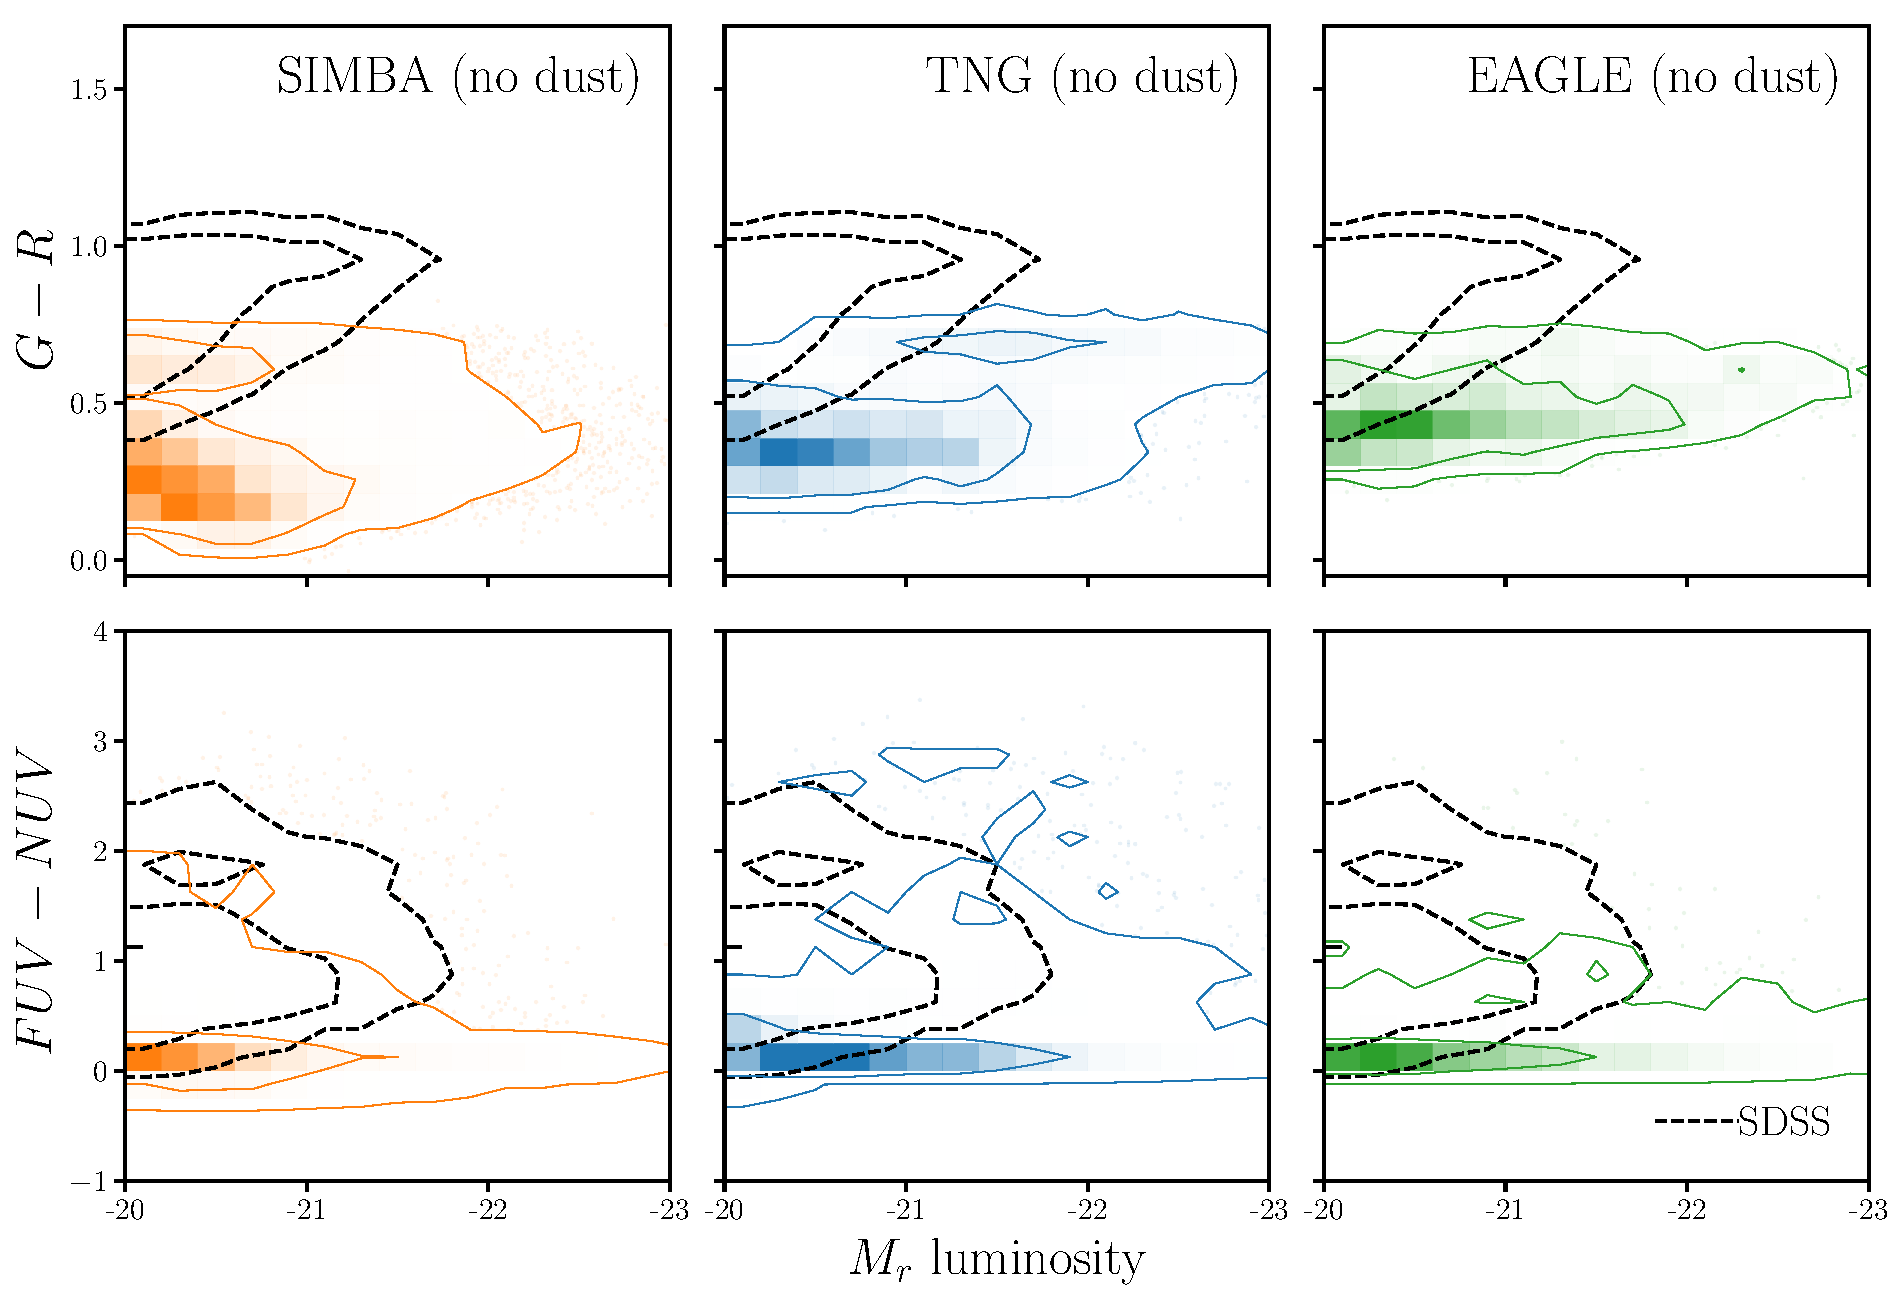
\includegraphics[width=\textwidth]{figs/observables.pdf} 
    \caption{We present the distributions of the main observables used
    throughout the paper for SDSS (left), SIMBA (center), and TNG (right)
    centrals. We do {\em not} include any prescription for dust for the
    simulated galaxies. The top panels
    present the $G-R$ versus $M_r$ color magnitude relations while the bottom
    panels present the $FUV-NUV$ versus $M_r$ relations. The observables for
    the SIMBA and TNG simulated galaxies are derived using forward modeling and
    are therefore consistent with SDSS measurements (Section~\ref{sec:fm}). The
    contours for SIMBA and TNG do not include galaxies with SFR$=0$, which we
    mark separately in black. Despite similar SMFs,  {\em the simulations
    without any dust prescription show stark differences with observations in
    the color-magnitude observable-space.} 
    }
\label{fig:obs}
\end{center}
\end{figure}
 
% --- methods ---  
\section{The Empirical Dust Attenuation Framework} \label{sec:dem}
\chedit{
    In this section, we describe the Empirical Dust Attenuation (\eda)
    framework and present the \eda~prescription we use in this work. 
    The \eda~is a flexible framework for applying dust attenuation curves to
    simulated galaxy populations.
    For each simulated galaxy, the \eda~assigns a dust attenuation
    curve that is parameterized as a function of the galaxy's properties 
    ($M_*$, ${\rm SSFR}$), the \eda~parameters, and randomly
    sampled inclination. With the \eda, we can apply a wide variety of dust
    attenuation that include correlation between dust attenuation and physical
    galaxy properties. 
}
% Later, we demonstrate that we can accurately reproduce SDSS observations with the \eda~and use it to test galaxy formation models and shed light on dust in galaxies. 

We begin by defining the dust attenuation curve, $A(\lambda)$, as 
\begin{equation} \label{eq:full_atten}
    F_o (\lambda) = F_i (\lambda) 10^{-0.4 A(\lambda)}
\end{equation}
where $F_o$ is the observed flux and $F_i$ is the intrinsic flux. We normalize
the attenuation to the $V$ band attenuation, 
\begin{equation} 
    A(\lambda) = A_V \frac{k(\lambda)}{k_V}
\end{equation}
so that $A_V$ determines the amplitude of the attenuation, while $k(\lambda)$
determines the wavelength dependence. 

\chedit{
    The \eda~framework assigns $A(\lambda)$ to every galaxy in the simulations
    using some flexible prescription. For the \eda~prescription in this work,
    we assign $A_V$ for each galaxy using the slab model, where $A_V$ is a
    function of galaxy inclination, $i$, and its optical depth,
    $\tau_V$~\citep[\eg][]{somerville1999, somerville2012}: 
}
\begin{equation} \label{eq:slab}
    A_V = -2.5 \log \left[ \frac{1 - e^{-\tau_V\,\sec i}}{\tau_V\,\sec i} \right].
\end{equation}
We parameterize $\tau_V$ using a linear $M_*$ and $\ssfr$ dependence: 
\begin{equation} \label{eq:tauv}
    \tau_V(M_*, \sfr) = \mtaum \log \left(\frac{M_*}{10^{10} M_\odot}\right) +
    \mtaus \log \left(\frac{\ssfr}{10^{-10}yr^{-1}}\right) + c_\tau.
\end{equation}
$\mtaum$, $\mtaus$, and $c_\tau$ represent the $M_*$ dependence, the $\ssfr$
dependence, and amplitude of $\tau_V$. Since $\tau_V$ is optical depth, we
impose a $\tau_V \ge 0$ limit.
For each galaxy, we uniformly sample $\cos i$ from 0 to 1. By sampling
$\cos i$, our \eda~prescription includes significant variance in
$A(\lambda)$ so galaxies with the same galaxy properties do not have the
same dust attenuation.

\chedit{
    Previous works, motivated by the fact that dust on small scales depend on
    local stellar and gas properties, have parameterized dust attenuation based
    on galaxy properties such as its gas density, gas metallicity, or star-gas
    geometry~\citep[\eg][]{somerville1999, somerville2012, steinacker2013,
    camps2015, narayanan2018, trayford2020, vogelsberger2020}. 
    The galaxies in the SIMBA, TNG, and EAGLE simulations, however, have
    substantially different gas masses and metallicites~\citep[][Maller \etal~in prep.]{dave2020}.  
    If we were to parameterize $\tau_V$ using these properties, the differences
    in them between the simulations would dominate any comparison of dust attenuation.
    Instead, we parameterize $\tau_V$ on correlation between dust attenuation
    and galaxy properties that have been established in observations~\citep[\eg~][]{garn2010, battisti2016, salim2020}.
    In Appendix~\ref{sec:slab}, we confirm the correlation between $A_V$ and
    the properties $M_*$ and $\ssfr$ using the \cite{salim2018} GSWLC2 sample
    (Figure~\ref{fig:dep}). 
    We therefore include in Eq.~\ref{eq:tauv} the correlation between $A_V$ and
    galaxy $M_*$ and $\ssfr$.
}


%\tksedit{
%The true properties of dust (grain size, temperature, and spatial
%distributions), determined by detailed dust growth and destruction processes,
%depend on local stellar and gas properties and the local star, gas, and dust
%geometries. 
%On scales relative for large-scale simulations the dust properties
%are expected to vary with gas density (alternatively gas column density or
%total gas mass), gas metallicity, and the relative star-gas geometry, and this
%is often used in estimations of attenuation of starlight by dust
%\citep[e.g.][]{somerville1999, somerville2012, steinacker2013, camps2015,
%narayanan2018, trayford2020, vogelsberger2020}.
%In this work we take an
%observation-centered approach to modeling dust and therefore base our model on
%observationally found relations between galaxy properties, $M_*$ and $\ssfr$,
%and dust attenuation. Moreover, the galaxy populations in the SIMBA, TNG, and
%EAGLE simulations show a variety of distributions in gas mass and gas
%metallicity which would dominate any inference we could make on the relation
%between dust and the galaxy population (e.g. \citealp{dave2020}, Maller et al.
%in prep.). We will explore the relation between our inferred attenuation and
%gas properties and compare in future work (Starkenburg et al. in prep.).
%}

\chedit{
    In Eq.~\ref{eq:slab}, we use the slab model because it provides a simple
    prescription for generating a distribution of $A_V$ that depends on
    randomly sampled $i$, with loose physical motivations.
    For star-forming galaxies, which typically have disc-like morphologies, the
    slab model produces $A_V$ that is correlated with $i$ in a way consistent
    with observations: edge-on galaxies have higher $A_V$ than face-on
    galaxies~\citep[\eg][]{conroy2010, wild2011, battisti2017, salim2020}.
    Nevertheless, the slab model is a naive approximation; in reality, $A_V$
    depends on the detailed star-to-dust geometry.
    Furthermore, all galaxies in the simulations are assigned $A_V$ from the
    slab model.
    For quiescent galaxies, which typically have elliptical morphologies, the
    slab model serves only as an \emph{empirical} prescription for statistically 
    sampling $A_V$. 
    However, the purpose of the~\eda~is to assign an accurate distribution of dust
    attenuation curves for the galaxy population --- \emph{not} to accurately
    model dust attenuation for individual galaxies.
    In this regard, we demonstrate that the slab model based \eda~can match the
    observed distribution of $A_V$, even for samples that include quiescent
    galaxies (Appendix~\ref{sec:slab}).
    Hence, the slab model provides a sufficient prescription for reproducing
    the $A_V$ distribution for all galaxies. 
}

For the wavelength dependence of the attenuation curve, $k(\lambda)$, we
use the \cite{noll2009} parameterization: 
\begin{equation} \label{eq:noll}
    k(\lambda) = \left(k_{\rm Cal}(\lambda) + D(\lambda)\right) \left(
    \frac{\lambda}{\lambda_V} \right)^\delta.
\end{equation}
Here $k_{\rm Cal}(\lambda)$ is the \cite{calzetti2001} curve: 
\[
    k_{\rm Cal}(\lambda) = 
    \begin{cases} 
        2.659 (-1.857 + 1.040/\lambda) + R_V, & 6300 A \le \lambda \le
        22000 A \\ 
        2.659 (-2.156 + 1.509/\lambda - 0.198/\lambda^2 + 0.011/\lambda^3) +
        R_V & 1200 A \le \lambda \le 6300 A
    \end{cases}
\]
where $\lambda_V = 5500 A$ is the $V$ band wavelength and $\delta$ is the slope
offset of the attenuation curve from $k_{\rm Cal}$. Since $\delta$ correlates 
with galaxy properties~\citep[\eg][; see also Appendix~\ref{sec:slab}]{wild2011, battisti2016, leja2017, salim2018},
we parameterize $\delta$ with a similar $M_*$ and $\ssfr$ dependence as
$\tau_V$:  
\begin{align} \label{eq:delta}
    \delta(M_*, \sfr) &= \mdeltam \log \left(\frac{M_*}{10^{10}
    M_\odot}\right) + \mdeltas \log \left(\frac{\ssfr}{10^{-10}yr^{-1}}\right)
    + c_\delta.
\end{align}
% Although a number of works have found correlation between the attenuation
% curve slope and inclination~\citep{wild2011, chevallard2013, battisti2017b},
% \cite{salim2020}, most recently, found that the driver of this trend is the
% relationship between $A_V$ and slope. We therefore do not include an
% inclination dependence in $\delta$. 
$D(\lambda)$ in Eq.~\ref{eq:noll} is the UV dust bump, which we parameter using
the standard Lorentzian-like Drude profile:
\begin{equation}
    D(\lambda) = \frac{E_b(\lambda~\Delta \lambda)^2}{(\lambda^2 -
    \lambda_0^2)^2 + (\lambda~\Delta \lambda)^2}
\end{equation}
where $\lambda_0$, $\Delta \lambda$, and $E_b$ are the central wavelength,
full width at half maximum, and strength of the bump, respectively. 
\chedit{
    We include the UV dust bump since we use UV color as one of our observables.
}
We assume fixed $\lambda_0 = 2175
A$ and $\Delta \lambda = 350A$. \cite{kriek2013} and \cite{tress2018} find
that $E_b$ correlates with the $\delta$ for star-forming galaxies $z\sim2$.
\cite{narayanan2018} confirmed this dependence in simulations. 
However, we assume a fixed relation between $E_B$ and $\delta$ from
\cite{kriek2013}: $E_b = -1.9~\delta + 0.85$. Allowing the slope and amplitude
of the $E_B$ and $\delta$ relation to vary does {\em not} impact our results;
however, we also do not derive any meaningful constraints on them. In
Table~\ref{tab:free_param}, we list and describe all of the free parameters of
the \eda. 

%In $\tau_V$ we include the correlation between $A_V$ and the galaxy's properties , found in both observations and simulations~\citep[\eg][]{narayanan2018, salim2020}. 


$\ssfr$ of galaxies are used to calculate $\tau_V$ and $\delta$ in
Eqs.~\ref{eq:tauv} and~\ref{eq:delta}. However, due to mass and temporal resolutions,
some galaxies in the simulations have $\sfr=0$ --- \ie~an unmeasurably low
SFR~\citep{hahn2019c}. They account for 17, 19, 9\% of galaxies
in SIMBA, TNG, and EAGLE, respectively. Since Eqs.~\ref{eq:tauv}
and~\ref{eq:delta} depend on $\log\ssfr$, they cannot be used in the equations
to derive $\tau_V$ and $\delta$ for these galaxies. To account for this issue,
we assign $\sfr_{\rm min}$, the minimum non-zero $\sfr$ in the simulations, to
$\sfr=0$ galaxies when calculating $\tau_V$ and $\delta$. For SIMBA, TNG, and
EAGLE, $\sfr_{\rm min}=0.000816$, $0.000268$, and $0.000707 M_\odot/yr$. Although 
this assumes that $\sfr=0$ galaxies have similar dust properties as the galaxies 
with $\sfr = \sfr_{\rm min}$, since the simulations have very low $\sfr_{\rm min}$ 
we expect galaxies with $\sfr = \sfr_{\rm min}$ to have little recent
star-formation and low gas mass, similar to $\sfr=0$ galaxies. 

%Since $\sfr=0$ galaxies do not account for a large fraction of our simulated galaxies, we directly sample their observables ($G, R, NUV$, and $FUV$) from the distribution of observables for SDSS quiescent galaxies. This way, we ensure that the attenuation of $\sfr=0$ galaxies does not impact the rest of the \eda~parameters. In Appendix~\ref{sec:res}, we discuss the resolution effects in more detail and demonstrate that our results are \emph{not} impacted by other prescriptions for attenuating $\sfr=0$ galaxies.

\chedit{
    In practice, to apply the \eda~to a simulated galaxy population, we first
    assign a randomly sampled $i$ to each galaxy ($\cos i$ uniformly sampled from 0 to 1).
    $\tau_V$ and $\delta$ are calculated for
    the galaxy based on its $M_*$,
    $\ssfr$ and the \eda~parameters. We then combine $A_V$ from $i$ and
    $\tau_V$ with $k(\lambda)$ from $\delta$ to determine $A(\lambda)$ for each
    galaxy.
} 
Afterwards, we attenuate the galaxy SEDs using Eq.~\ref{eq:full_atten} and use
the attenuated SEDs to calculate the observables: $g, r, NUV$, and $FUV$
absolute magnitudes. 
\ch{
    In Figure~\ref{fig:dem_av}, we present attenuation curves, $A(\lambda)$,
    generated by the \eda~for galaxies with different $\sfr$ and $M_*$ values.  
    We include star-forming galaxies with $\{M_*, \sfr\} = \{10^{10}M_\odot,
    10^{0.5}M_\odot/yr\}$ (blue), $\{10^{11}M_\odot, 10^{1} M_\odot/yr\}$
    (green) and a quiescent galaxy with $\{10^{11}M_\odot, 10^{-2}M_\odot/yr\}$
    (red).
    We use an arbitrarily set of \eda~parameters ($\mtaum, \mtaus, c_\tau,
    \mdeltam, \mdeltas, c_\delta$) within the prior range listed in
    Table~\ref{tab:free_param}. 
    We set $i=0$ (edge-on) for all $A(\lambda)$ in Figure~\ref{fig:dem_av} for
    simplicity.
    In practice the \eda~uniformly samples $\cos i$ from 0 to 1 for each galaxy.
}
For comparison, we include the \cite{calzetti2001} attenuation curve. Even when
we set $i=0$, the \eda~produces attenuation curves with a wide range
of amplitude and slope to galaxies based on their physical properties. 

\begin{figure}
\begin{center}
    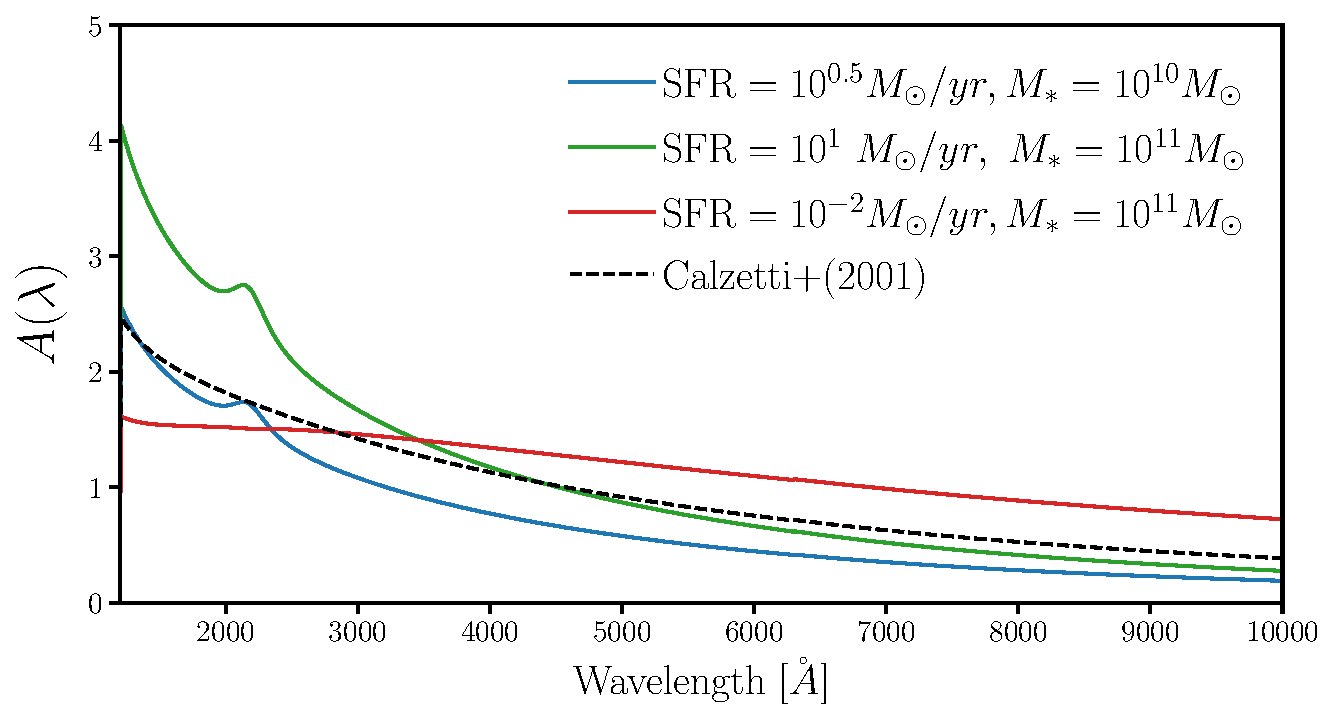
\includegraphics[width=0.6\textwidth]{figs/dems.pdf}
    \caption{\label{fig:dem_av}
    \chedit{
        Attenuation curves, $A(\lambda)$, assigned by our Empirical Dust
        Attenuation (\eda) prescription to edge-on galaxies with different $\sfr$ and
        $M_*$ values for an arbitrary set of \eda~parameters. We include
        $A(\lambda)$ for star-forming galaxies with $\{M_*, \sfr\} =
        \{10^{10}M_\odot, 10^{0.5}M_\odot/yr\}$ (blue), $\{10^{11}M_\odot, 10^{1}
        M_\odot/yr\}$ (green) and a quiescent galaxy with $\{10^{11}M_\odot,
        10^{-2}M_\odot/yr\}$ (red). We set $i=0$ for
        all the galaxies in the figure for simplicity but in practice the
        \eda~uniformly samples $\cos i$ from 0 to 1 for each galaxy.
        For comparison, we include the \cite{calzetti2001} attenuation curve.
        {\em The \eda~provides a flexible prescription for assigning dust
        attenuation to galaxies based on their inclination, physical properties
        ($M_*$ and $\ssfr$), and the \eda~parameters.}
    }
    } 
\end{center}
\end{figure}


%%%%%%%%%%%%%%%%%%%%%%%%%%%%%%%%%%%%%%%%%%
% table of free parameters
%%%%%%%%%%%%%%%%%%%%%%%%%%%%%%%%%%%%%%%%%%
\begin{table}
    \caption{Free parameters of the Empirical Dust Attenuation Model}
    \begin{center}
        \begin{tabular}{ccc} \toprule
            Parameter & Definition & prior\\[3pt] \hline\hline
            %\multicolumn{3}{c}{DEM with slab model}\\ \hline
            $\mtaum$ & $M_*$ dependence of the optical depth, $\tau_V$ & flat $[-5., 5.]$\\
            $\mtaus$ & $\ssfr$ dependence of $\tau_V$  & flat $[-5., 5.]$\\
            $c_{\tau}$ & amplitude of $\tau_V$ & flat $[0., 6.]$\\
            %\hline
            %\multicolumn{3}{c}{DEM with $\mathcal{N}_T$ model}\\ \hline
            %$m_{\mu,1}$ & Slope of the $\log M_*$ dependence of optical depth,
            %$\tau_V$ & flat $[-5., 5.]$\\
            %$m_{\mu,2}$ & Slope of the $\log {\rm SFR}$ dependence of optical
            %depth, $\tau_V$ & flat $[-5., 5.]$\\
            %$c_{\mu}$ & amplitude of the optical depth, $\tau_V$ & flat $[0., 6.]$\\ 
            %$m_{\sigma,1}$ & Slope of the $\log M_*$ dependence of optical depth, $\tau_V$ & flat $[-5., 5.]$\\
            %$m_{\sigma,2}$ & Slope of the $\log {\rm SFR}$ dependence of optical depth, $\tau_V$ & flat $[-5., 5.]$\\
            %$c_{\sigma}$ & amplitude of the optical depth, $\tau_V$ & flat $[0.1, 3.]$\\ 
            %\hline
            $\mdeltam$ & $M_*$ dependence of $\delta$, the attenuation curve slope offset & flat $[-4., 4.]$\\
            $\mdeltas$ & $\ssfr$ dependence of $\delta$ & flat $[-4., 4.]$\\
            $c_{\delta}$ & amplitude of $\delta$ & flat $[-4., 4.]$\\
            %$f_{\rm neb}$ & nebular attenuation fraction & flat $[1., 4.]$\\
            \hline
        \end{tabular} \label{tab:free_param}
    \end{center}
\end{table}
%%%%%%%%%%%%%%%%%%%%%%%%%%%%%%%%%%%%%%%%%%


\section{Likelihood-Free Inference: Approximate Bayesian Computation} \label{sec:abc}
\chedit{
    With our forward model, which includes the \eda~prescription for dust
    attenuation, we can now generate synthetic observations for simulated
    galaxies and make an ``apples-to-apples'' comparison to SDSS. Next, we want
    to use this comparison to infer the posterior probability distribution of
    the \eda~parameters. Typically in astronomy, this inference is done
    assuming a Gaussian likelihood to compare the ``summary statistic''
    (\eg~SMF) of the model to observations and some sampling method (\eg~Markov
    Chain Monte Carlo) to estimate the posterior distribution. The functional form of the
    likelihood, however, depends on the summary statistic and assuming an
    incorrect form of the likelihood can significantly bias the inferred
    posteriors~\citep[\eg][]{hahn2019}. In this work, we use the optical and UV
    color-magnitude relations as our summary statistic. Since the statistic is
    three-dimensional histogram, its likelihood is {\em not} Gaussian but
    rather a Poisson distribution.
}

\chedit{
    Rather than \emph{incorrectly} assuming a Gaussian likelihood or attempting
    to estimate the true Poisson likelihood of the optical and UV
    color-magnitude relations, we use Approximate Bayesian Computation~\citep[hereafter
    ABC;][]{diggle1984, tavare1997, pritchard1999, beaumont2009, delmoral2012}
    for our inference. 
}
ABC is a likelihood-free (or ``simulation-based'') parameter inference
framework that approximates the posterior probability distribution, $p(\theta\given{\rm data})$, without
requiring evaluations of the likelihood.  Instead, ABC only requires a forward
model of the observed data, a prior that can be sampled, and a distance metric
that quantifies the ``closeness'' to the observed data. 
\chedit{
    Since ABC does not require evaluating the likelihood, it does not assume
    any functional form of the likelihood and so we avoid any biases from such
    assumptions. Furthermore, it also allows us to infer the posterior using
    summary statistics with likelihoods that are difficult or intractable to
    directly estimate~\citep{hahn2017a}.
}

In the simplest version of ABC, with a rejection sample
framework~\citep{pritchard1999}, a proposal set of parameter values are drawn
from the prior. The forward model is run with the proposal parameter values.
\chedit{
    The output of the forward model is then compared to the observed data using
    a distance metric that quantifies the ``closeness'' of the forward model
    output to the observed data. 
}
If the distance is within some small threshold, we keep the proposed
parameters; otherwise, we discard them.  Proposals are
drawn until enough pass the threshold to sample the posterior. A
rejection sampling framework requires a large number of evaluations of the
forward model, which
can be computationally costly. Many variations of ABC with more efficient
sampling strategies have now been applied to astronomy and
cosmology~\citep[\eg][]{cameron2012, weyant2013, ishida2015, lin2016, alsing2018}.
Among these methods, we use ABC with Population Monte Carlo (PMC) 
importance sampling~\citep{hahn2017a, hahn2017b, hahn2019a}.

ABC-PMC begins with an arbitrarily large threshold $\epsilon_1$ and $N$ proposals 
$\bar{\theta}_1$ sampled from the prior distribution. Each proposal is
assigned a weight $w^i_1 = 1/N$. Then for subsequent iterations ($n > 1$), the 
threshold, $\epsilon_n$, is set to the median distance of the previous iteration's
proposals. New proposals are drawn from the previous iteration's proposals perturbed 
by a kernel and kept if their distance is blelow $\epsilon_n$. This is repeated
until we assemble a new set of $N$ proposals $\bar{\theta}_n$. The entire
process is repeated for the next iteration until convergence is confirmed. 
We use the Python implementation of
\cite{akeret2015}\footnote{https://abcpmc.readthedocs.io/en/latest/index.html}.
For further details on the ABC-PMC implementation, we refer readers to \cite{hahn2017b}
and \cite{hahn2019a}.

\begin{figure}
\begin{center}
    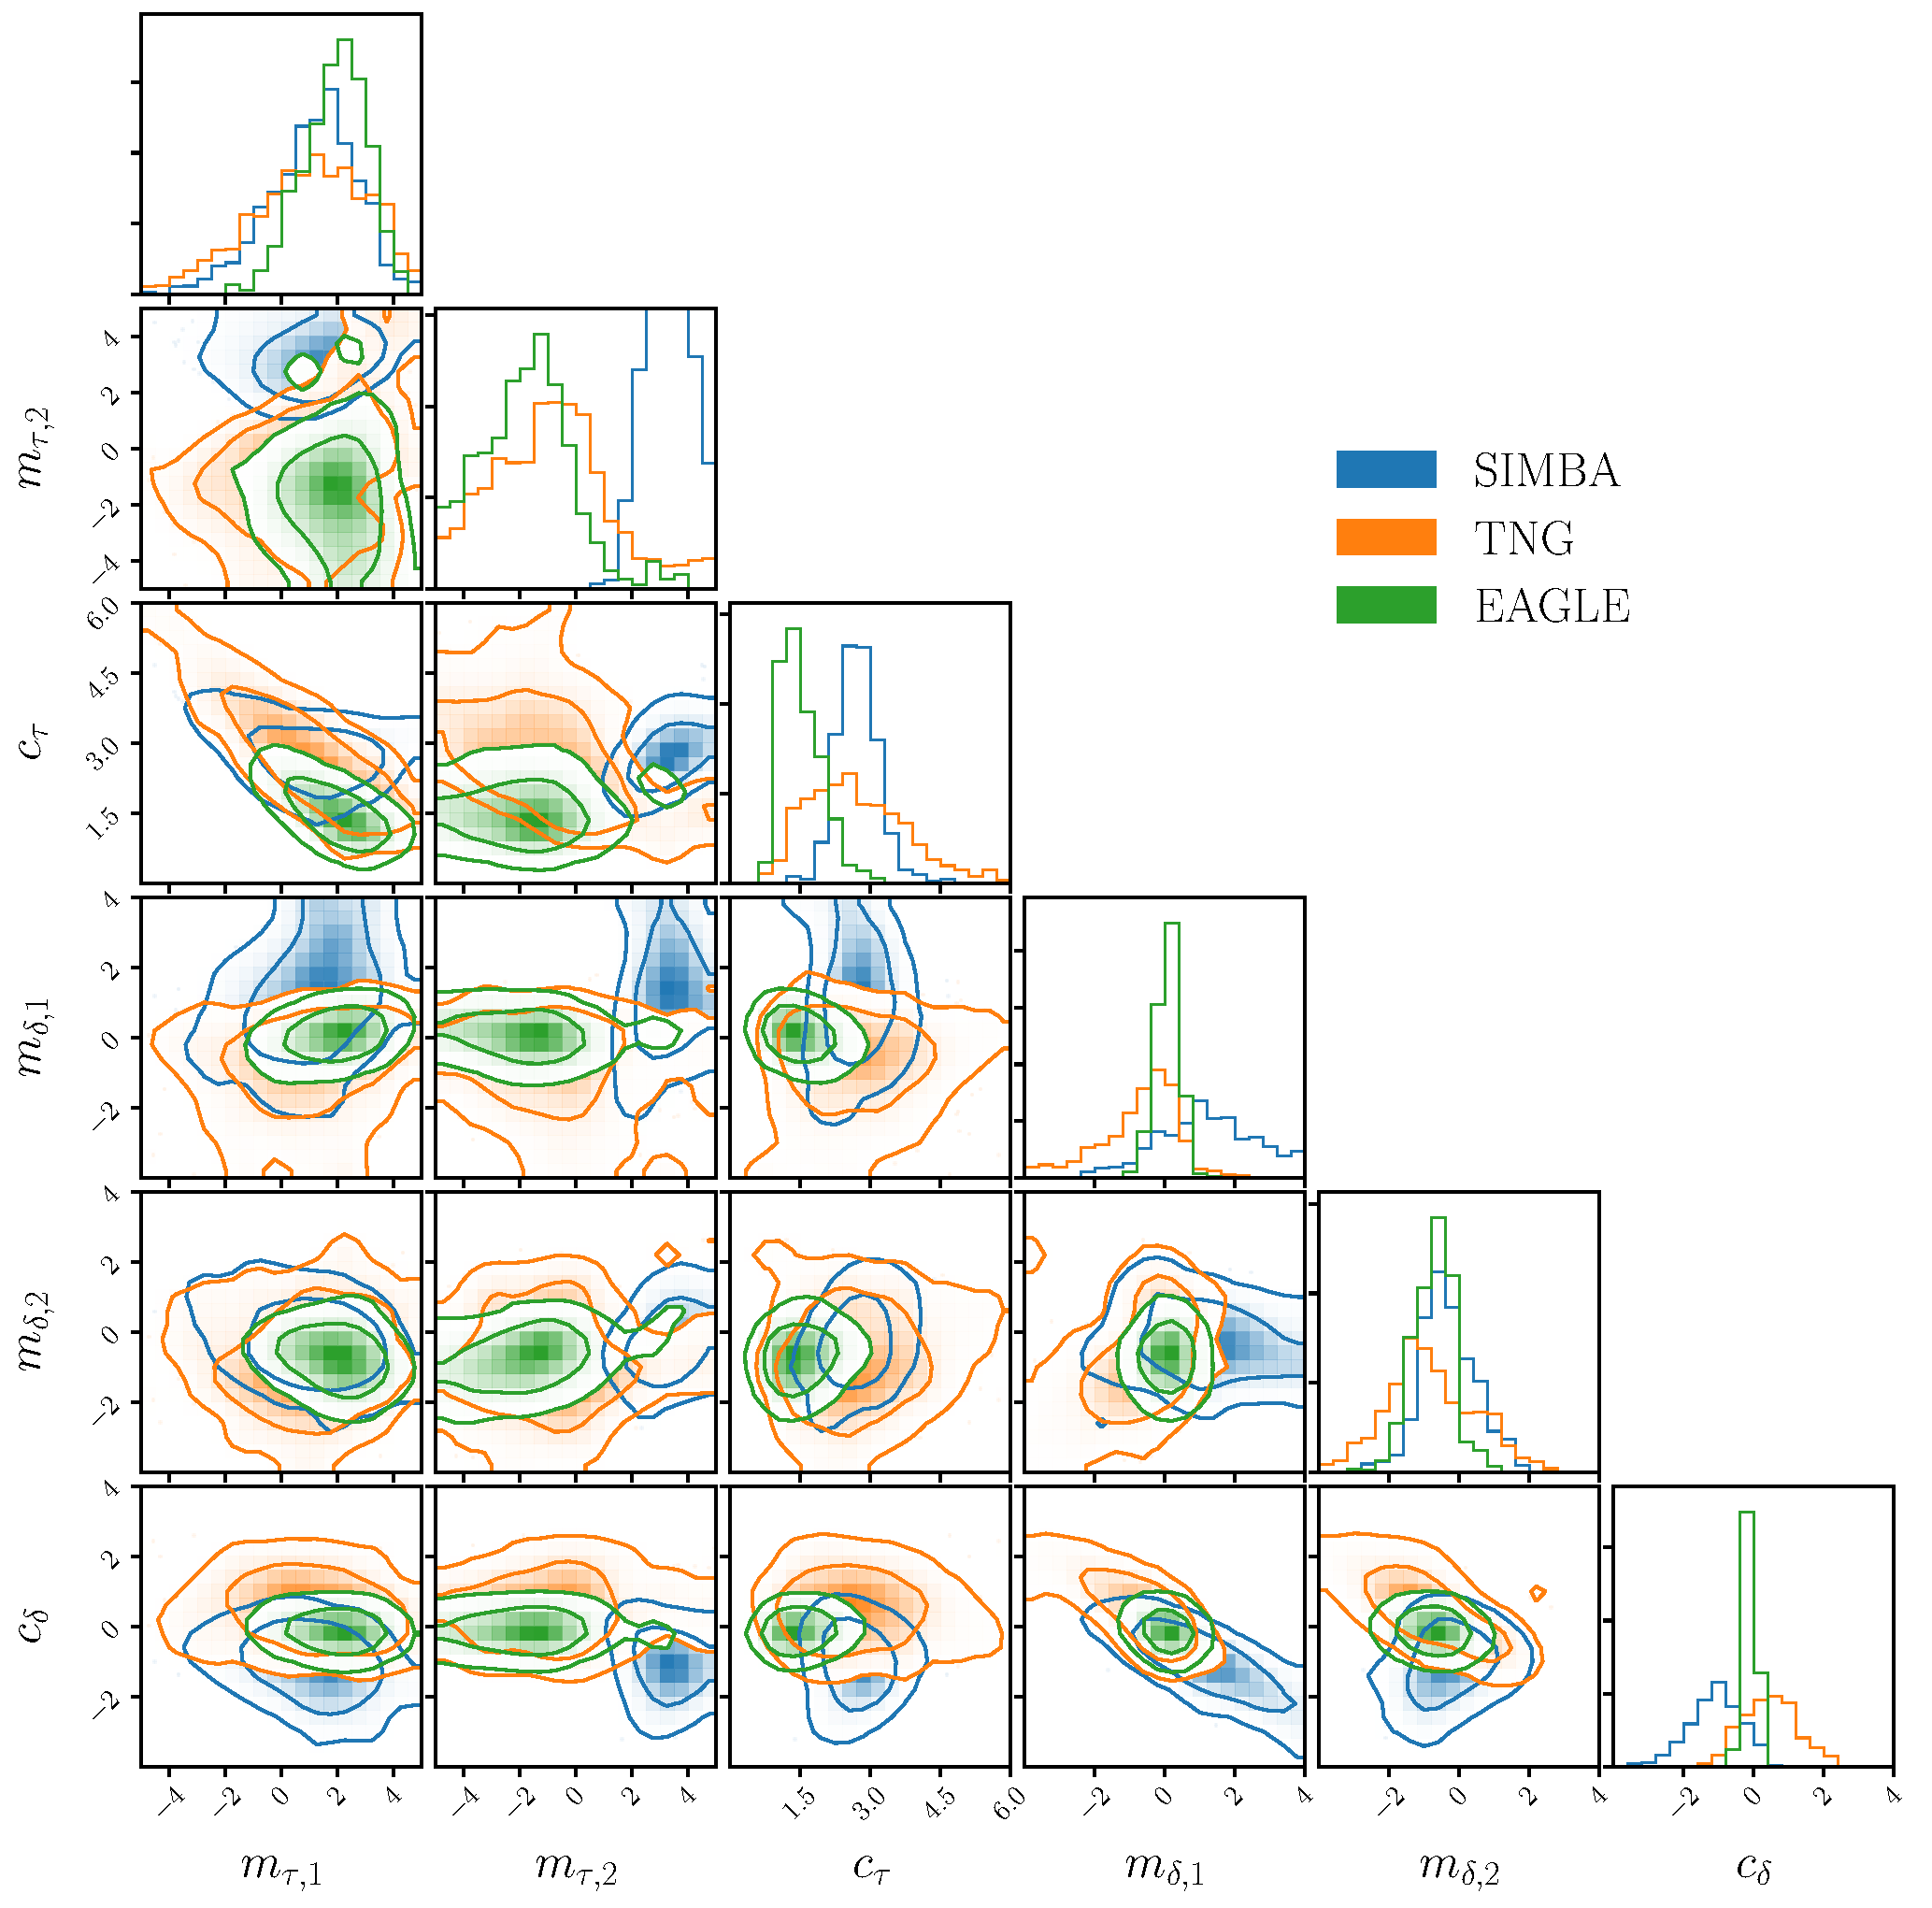
\includegraphics[width=\textwidth]{figs/abc.pdf}
    \caption{\label{fig:abc}
    Posterior distributions of the \eda~parameters for the SIMBA (orange), TNG
    (blue), and EAGLE (green) hydrodynamical simulations. The contours mark the $68$
    and $95$ percentiles of the distributions. The posteriors are derived using the
    likelihood-free inference method: Approximate Bayesian Computation with
    Population Monte Carlo (Section~\ref{sec:abc}). We focus on the
    \eda~posteriors for TNG and EAGLE since the \eda~struggles to reproduce
    SDSS observations with SIMBA, which predicts an overabundance of starburst
    galaxies. Based on the posteriors, we find that \emph{galaxies with higher
    $M_*$ have overall higher dust attenuation and galaxies with higher $\ssfr$
    have steeper attenuation curves.}
    }
\end{center}
\end{figure}

\chedit{
    In this work, we use ABC-PMC with uninformative uniform priors on each of
    the \eda~parameters and choose ranges that encompass constraints in the
    literature.
}
The prior ranges of $\mtaum, \mtaus, c_\tau$ are chosen to
conservatively include the $A_V$ range and $M_*$ and $\sfr$ dependence of
\cite{narayanan2018} and \cite{salim2020}. Meanwhile, the prior ranges of 
$\mdeltam, \mdeltas, c_\delta$ are chosen to conservatively include the $\delta$
range and $M_*$ and $\sfr$ dependence of \cite{leja2017} and \cite{salim2018}. 
We list the range of the priors in Table~\ref{tab:free_param}. 
\chedit{
    For our forward model, we use the model described in
    Section~\ref{sec:fm}: we construct SEDs for every simulated galaxies from
    the hydrodynamic simulations, apply dust attenuation with our
    \eda, calculate the observables ($M_r$, $\gr$, and $\fnuv$),
    add uncertainties to them, and apply a $M_r < -20$ completeness 
    limit. 
    We use the optical and UV color-magnitude relation, $(\gr)- M_r$ and
    $(\fnuv)-M_r$ as our summary statistic to fully exploit the $(M_r, \gr,
    \fnuv)$ observational-space. We measure the color-magnitude relations by
    calculating the number density in bins of $(\gr, \fnuv, M_r)$ with widths
    $(0.0625, 0.25, 0.5)$ mags. For our distance metric, $\rho$, we use the L2
    norm between the summary statistics of 
    the SDSS observation, $X^{\rm SDSS}$ and of our forward model, $X^{\rm
    FM}(\theta_{\rm \eda})$: 
}
\begin{equation} \label{eq:distance}
    \rho(\theta_{\rm \eda}) = \left[X^{\rm SDSS} - X^{\rm FM}(\theta_{\rm
    \eda}) \right]^2.
\end{equation}
In Figure~\ref{fig:abc}, we present the posterior distributions of the \eda~parameters
derived using ABC-PMC for the SIMBA (orange), TNG (blue), and EAGLE (green) hydrodynamical 
simulations. The contours mark the $68$ and $95$ percentiles of the distributions. 

% --- results ---  
\begin{figure}
\begin{center}
    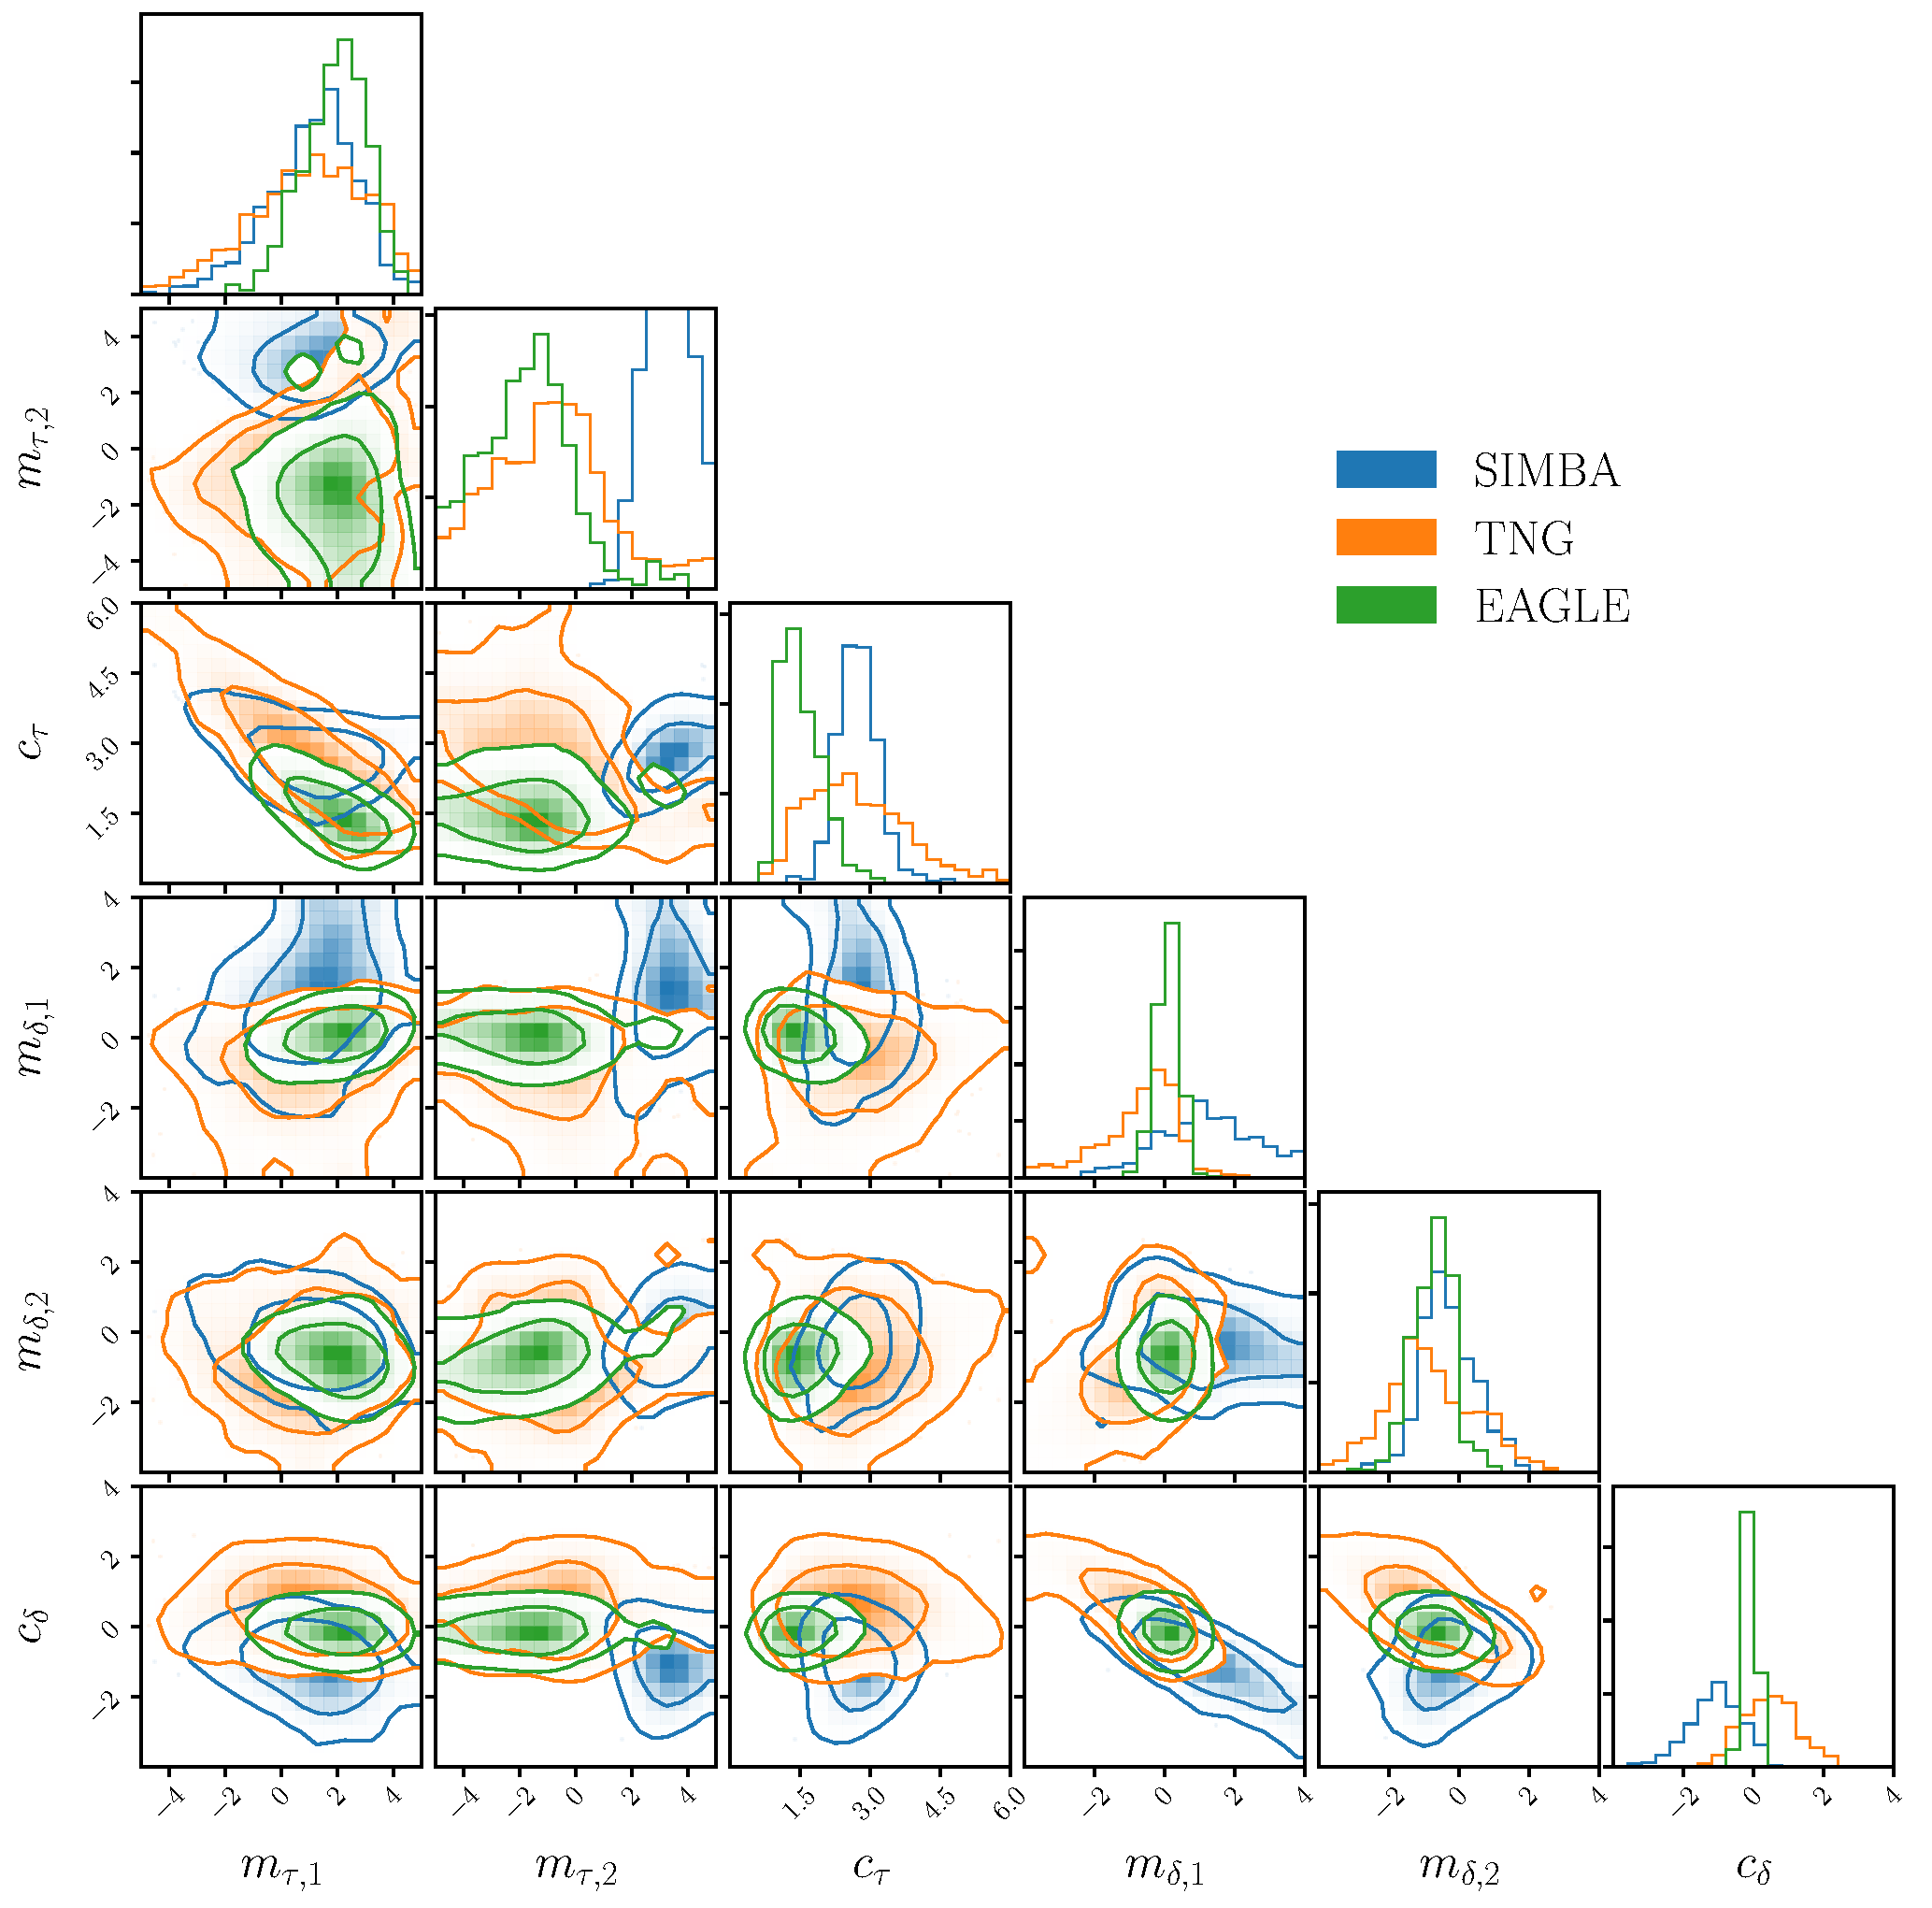
\includegraphics[width=\textwidth]{figs/abc.pdf}
    \caption{\label{fig:abc}
    Posterior distributions of our DEM parameters for the SIMBA (orange), TNG
    (blue), and EAGLE (green) hydro simulations. The contours mark the $68\%$
    and $95\%$ confidence intervals. We describe the parameters in
    Section~\ref{sec:dem} and Table~\ref{tab:free_param} and derive these
    posteriors using Approximate Bayesian Computation (Section~\ref{sec:abc}). 
    In all simulations, dust attenuation increases for higher $M_*$ galaxies 
    ($m_{\tau,M_*} \sim 2$). The simulations also have consistent optical 
    depth amplitudes ($c_\tau$). However, the ${\rm SFR}$ dependence of
    $\tau_V$ is different among the simulations. For TNG and EAGLE,
    star-forming galaxies have lower $\tau_V$; for SIMBA quiescent galaxies
    have lower $\tau_V$. Meanwhile, for the slope offset of the attenuation
    curve, $\delta$, we find little $M_*$ and ${\rm SFR}$ dependence in the
    simulations and that the amplitude ($c_\tau$) is consistent with 0. 
    }
\end{center}
\end{figure}

\begin{figure}
\begin{center}
    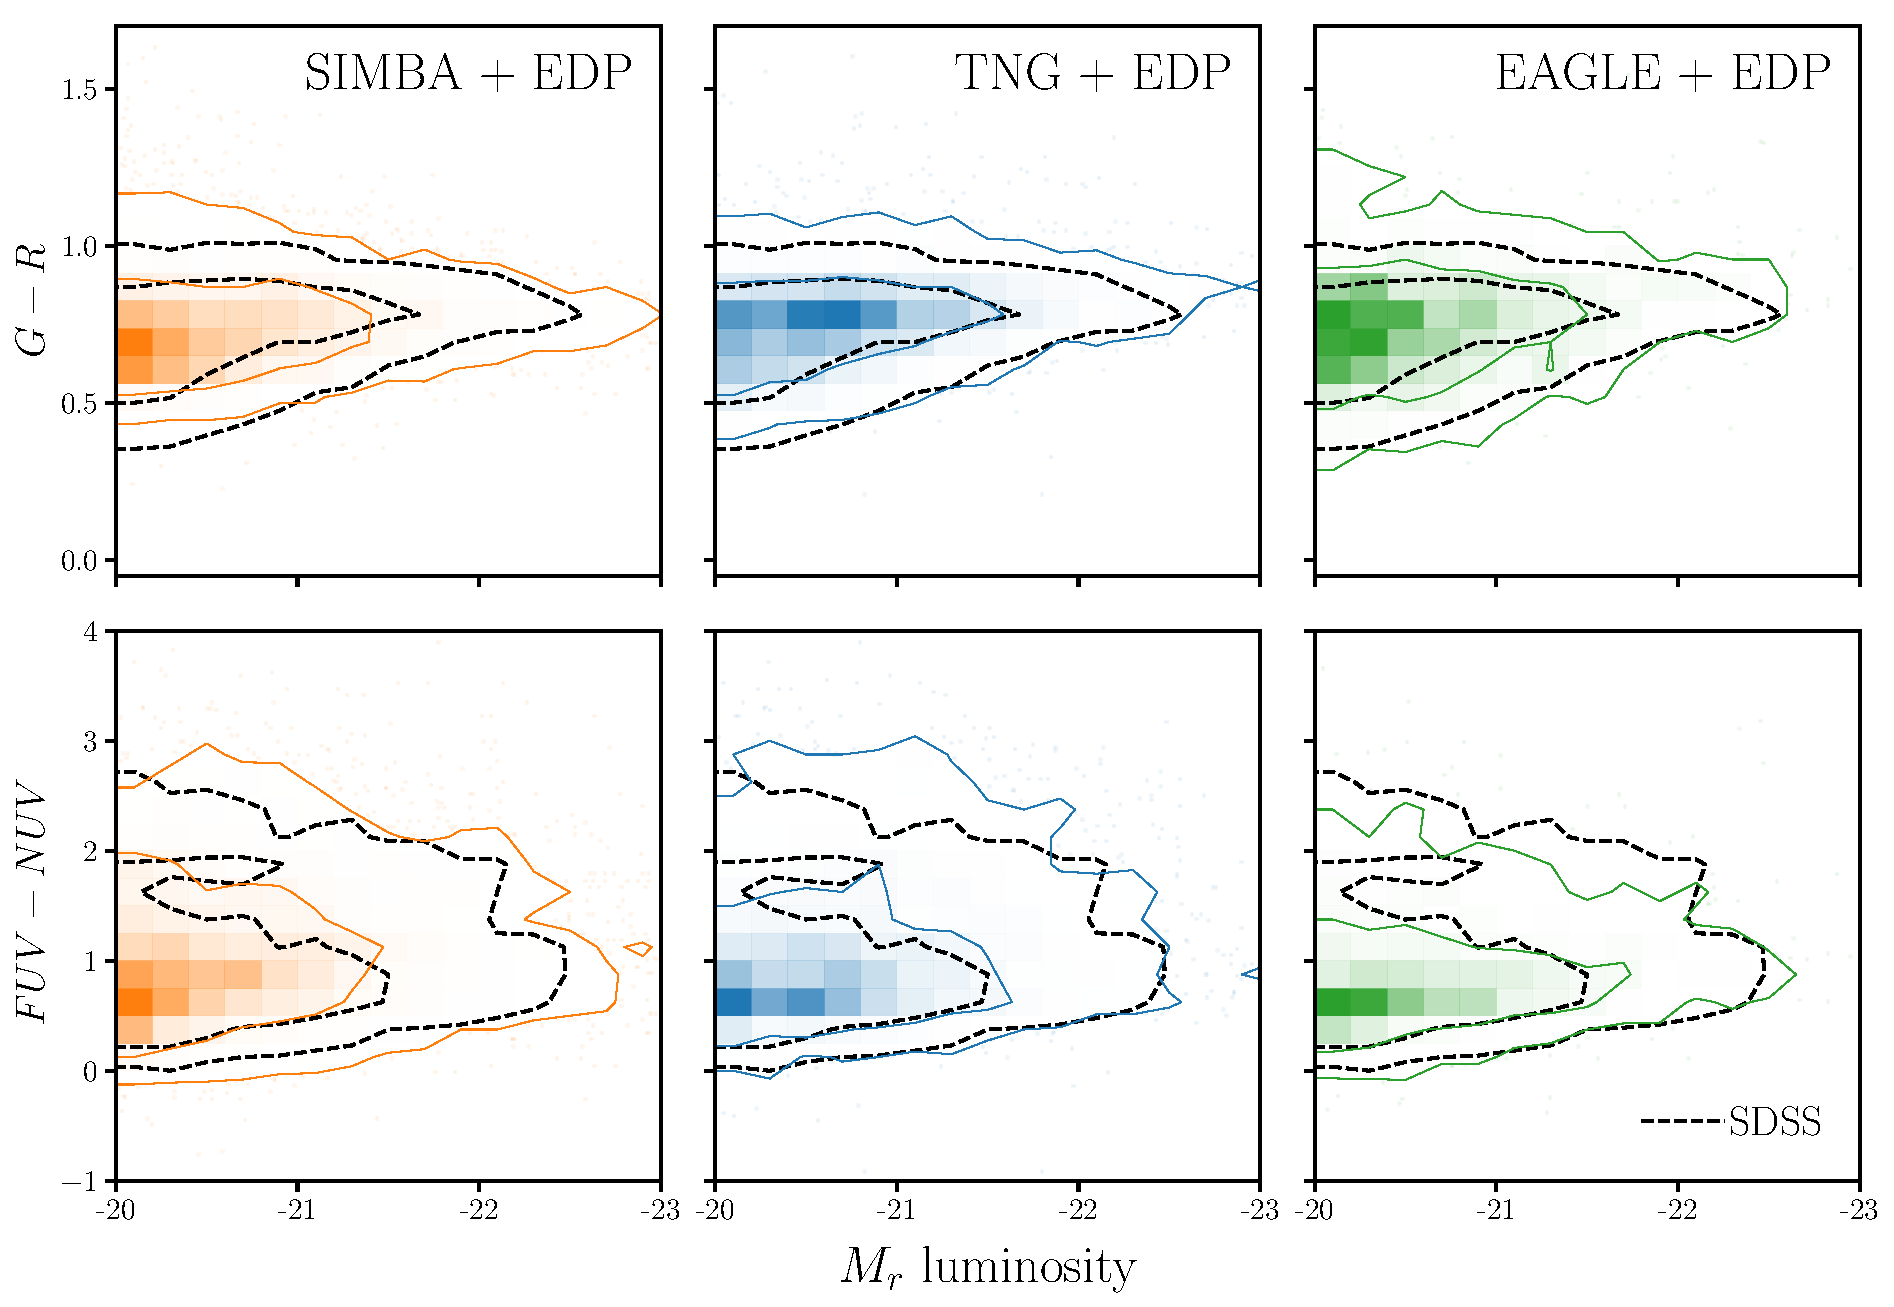
\includegraphics[width=0.9\textwidth]{figs/abc_observables.pdf}
    \caption{\label{fig:dem}
    $(G-R) - M_r$ color-magnitude (top panels) and $(FUV-NUV) - M_r$ (bottom
    panels) relations predicted by the median DEM posteriors for the SIMBA
    (orange), TNG (blue), and EAGLE (green) hydro simulations. For comparison, 
    we include the observables for SDSS in the left-most panel
    (Section~\ref{sec:obs}). The median posterior DEMs produce dramatically 
    different observables than when we do not include any dust prescription
    (Figure~\ref{fig:obs}). Hence, dust must be account for when interpreting 
    and comparing simulations. Moreover, with the DEMs, all three simulations
    produce observables consistent with SDSS. Since different simulations can 
    produce reproduce observations by varying dust, dust significantly limits
    our ability to constrain the physical processes that go into galaxy
    simulations. 
    }
\end{center}
\end{figure}


\begin{figure}
\begin{center}
    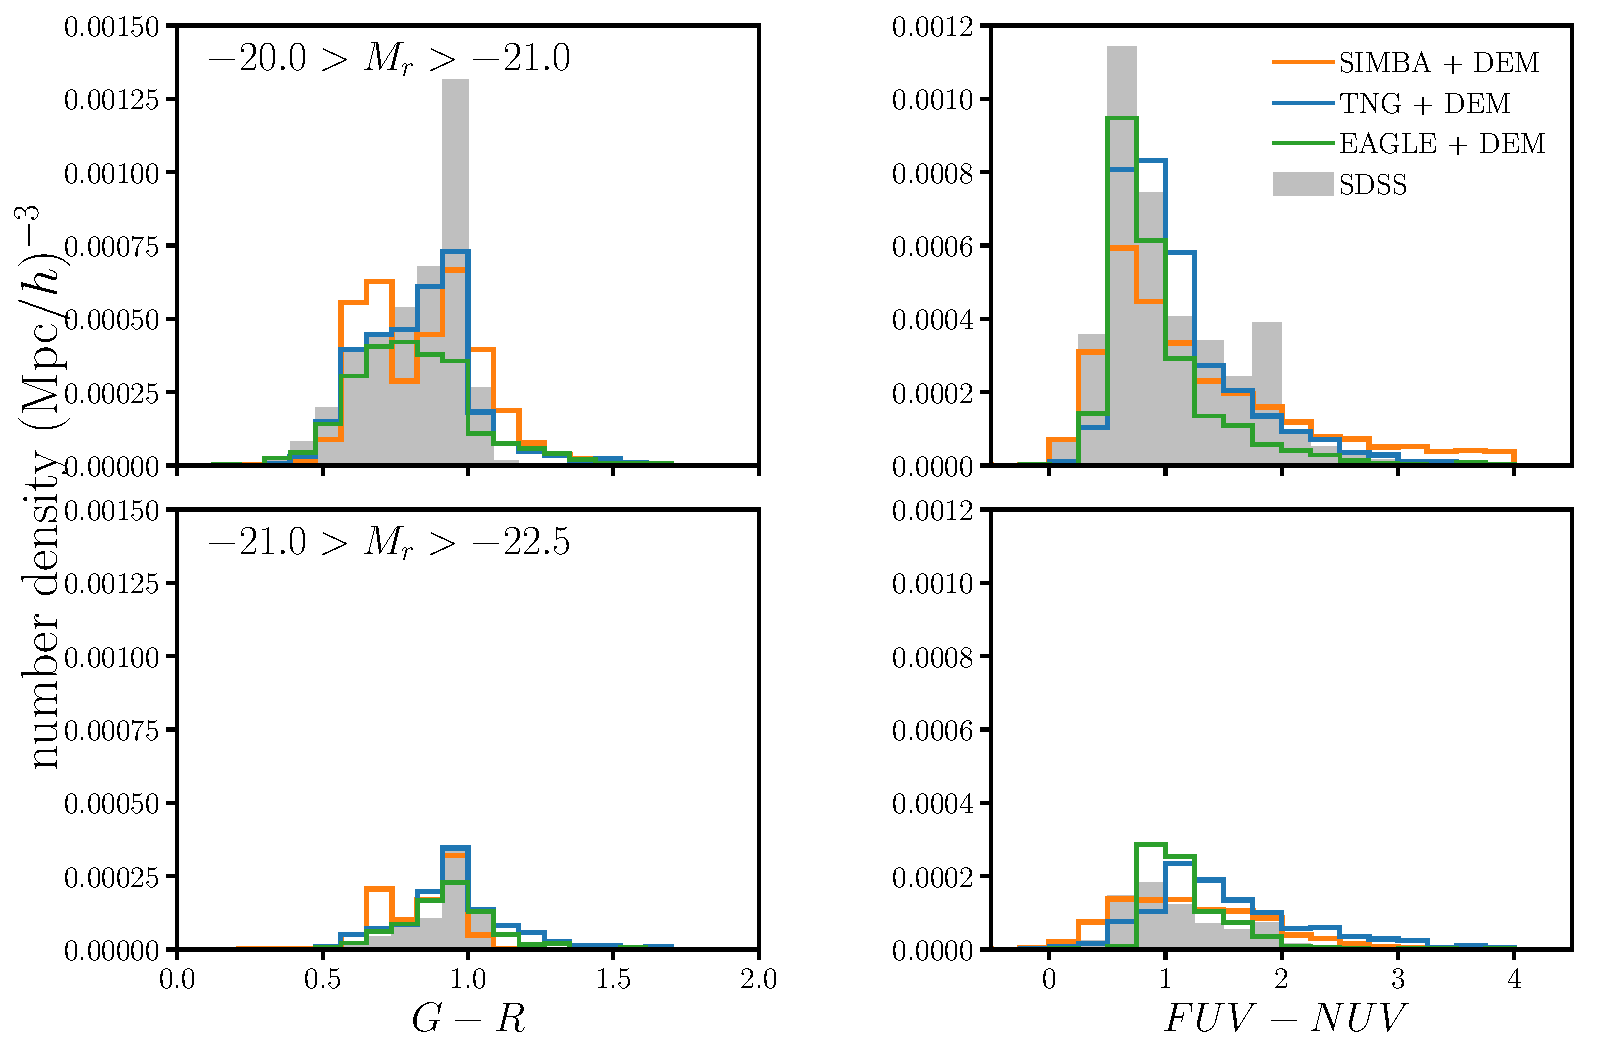
\includegraphics[width=0.85\textwidth]{figs/abc_observables_mr_bin.pdf}
    \caption{\label{fig:demcloseup}
    $G-R$ (left) and $FUV-NUV$ (right) number density distributions for the DEM
    models of the SIMBA (orange), TNG (blue), and EAGLE (green) simulations in
    two $M_r$ bins: $-20 > M_r > -21$ (top panels) and $-21 > M_r > -22.5$
    (bottom panels).  Each of the DEM models are run using the median posterior
    parameter values. In comparison to SDSS (grey shaded), the DEM models predict 
    consistent red sequence and blue cloud positions in the $G-R$ distributions, 
    $FUV-NUV$ peak positions, and number density. {\em Overall the DEM
    models for SIMBA, TNG, and EAGLE produce observables are in good agreement 
    with SDSS.}
    }
\end{center}
\end{figure}



\begin{figure}
\begin{center}
    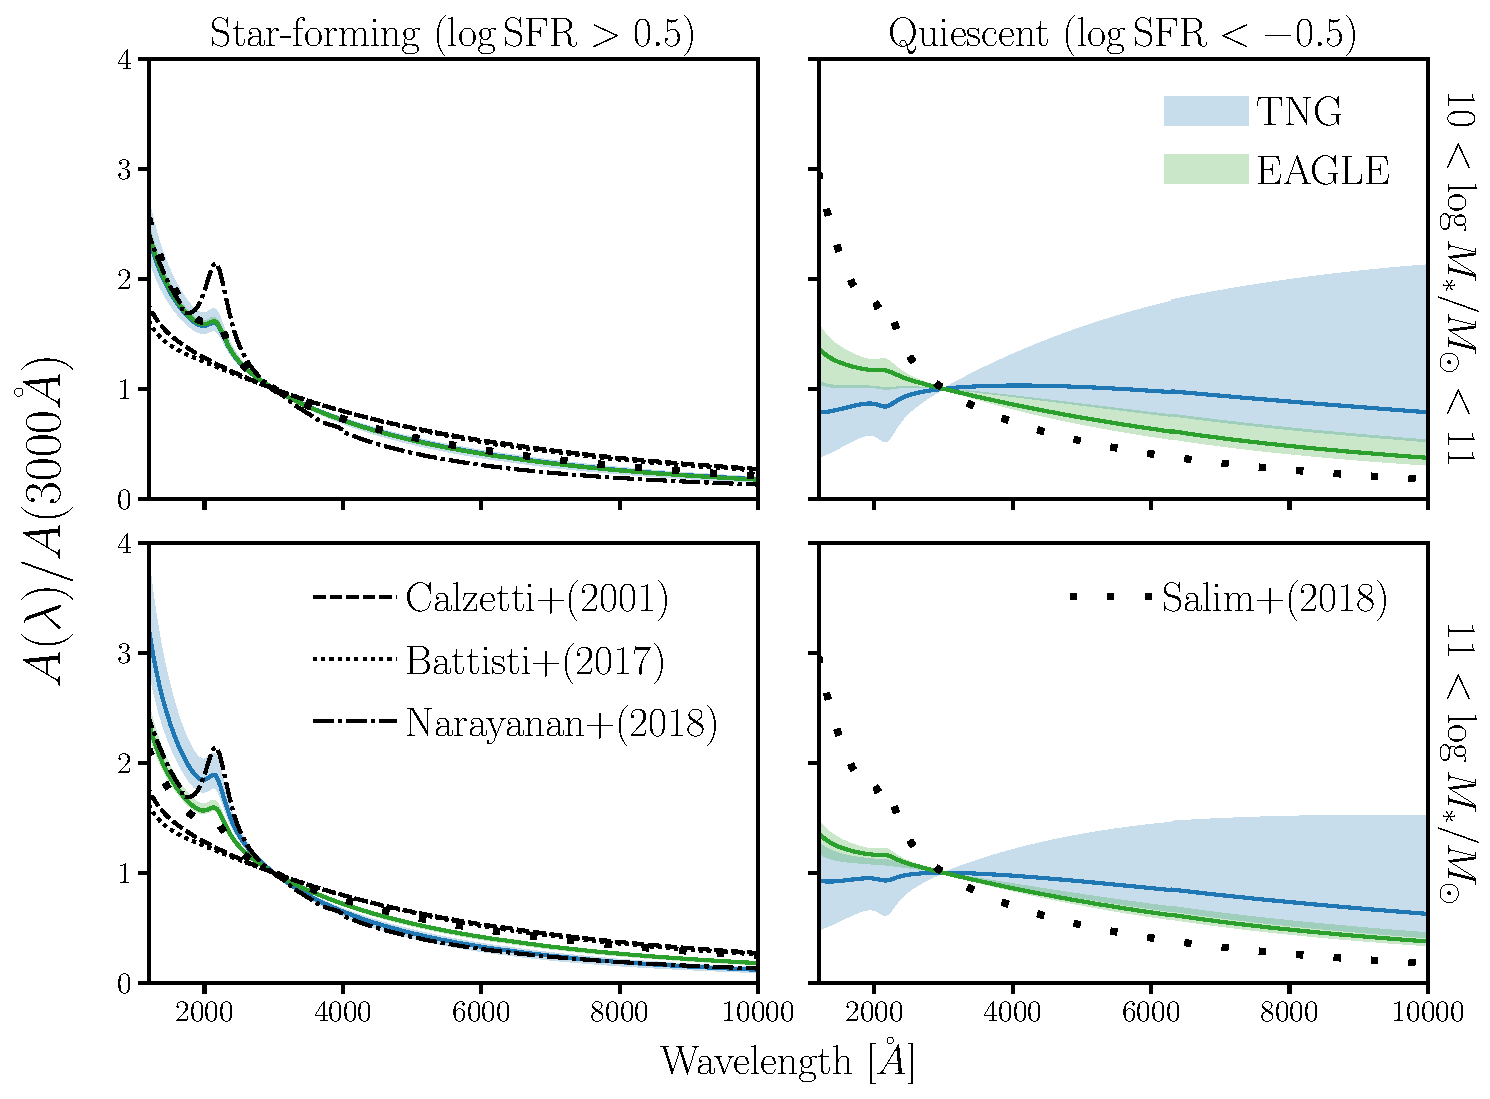
\includegraphics[width=0.85\textwidth]{figs/abc_attenuation.pdf}
    \caption{\label{fig:atten}
    }
\end{center}
\end{figure}

\section{Results} \label{sec:results}
We present the posterior distributions of the DEM parameters for the SIMBA
(orange), TNG (blue), and EAGLE (green) hydro simulations in
Figure~\ref{fig:abc}. The DEM parameters include $\mtaum$, $\mtaus$, and
$\ctau$, which parameterize the $M_*$ dependence, $\sfr$ dependence, and 
amplitude of $\tau_V$, the $V$-band optical depth. $\tau_V$ dictates the
overall strength of the dust attenuation. They also include $\mdeltam$,
$\mdeltas$, and $\cdelta$, which parameterize the $M_*$ dependence, $\sfr$ dependence,
and amplitude of $\delta$, the slope offset of the attenuation curve
(Section~\ref{sec:dem} and Table~\ref{tab:free_param}). The posteriors 
are derived using ABC (Section~\ref{sec:abc}) and the contours mark the 
$68\%$ and $95\%$ confidence intervals. 

In addition, we present the observables predicted by the DEM with median of the
posteriors for the SIMBA (orange), TNG (blue), and EAGLE (green) simulations 
in Figure~\ref{fig:dem}. We include the SDSS observables for comparison
(black dashed; Section~\ref{sec:obs}). The top panels present the $(G-R) - M_r$ 
color-magnitude relations while the bottom panels present the $(FUV-NUV) - M_r$
relations. Without any dust prescriptions, we found that simulations predict
dramatically different observables than SDSS (Figure~\ref{fig:obs}). 
\ch{something about clear bimodality with the red sequence and blue cloud} 
In contrast, {\em using DEMs we produce $(G-R) - M_r$ and $(FUV-NUV) - M_r$
relations consistent with SDSS for all of the simulations}. 

We examine the observables more closely in Figure~\ref{fig:demcloseup}, where
we present the $G-R$ (left) and $FUV-NUV$ (right) distributions in $M_r$ 
bins for the DEM models of the SIMBA (orange), TNG (blue), and EAGLE (green) 
simulations. The top panels contain galaxies with $-20 > M_r > -21$ and the 
bottom panels contain galaxies with $-21 > M_r > -22.5$. In each panel we 
include the SDSS distributions for comparison (grey shaded). These distributions are 
number densities. The positions of the red sequence and blue cloud in the $G-R$
distributions for the DEM models are consistent with the SDSS distribution. 
They also produce $FUV_NUV$ distributions with peaks consistent with
observations. We also find good agreement in the overall normalization
(number density), especially for the $-20 > M_r > -21$ bin. 

There are also a few discrepancies between the DEM models and SDSS observations. 
First, the red sequence in the observed $G-R$ distribution has a sharp red color 
cut-off.  In contrast, we do not find as sharp of a $G-R$ cut off in the DEM models, 
and find a small fraction of galaxies redder than observations. 
Furthermore, while the DEM models for TNG and EAGLE agree with SDSS, the DEM
model for SIMBA overpredicts blue galaxies. \ch{what do we want to do with
SIMBA?} We also find that the TNG and EAGLE DEM models slightly overpredict 
galaxies in the higher luminosity bin and produce a broader $G-R$ distribution.
Nonetheless, Figure~\ref{fig:demcloseup} demonstrates that overall the DEM
models for SIMBA, TNG, and EAGLE produce observables are in good agreement 
with SDSS.

% comparison to literature 
% First EAGLE
Previous works in the literature have also presented models that predict colors
and luminosities for different simulations and dust models and compared them to
observations. For instance, \cite{trayford2015} calculate colors and luminosities 
for $z=0.1$ galaxies using EAGLE with the {\sc GALAXEV} population synthesis models 
and a two-component screen model for dust. Compared to GAMA observations, their
model produces a bluer red sequence and overpredicts luminous blue galaxies~\citep[][Figure
5]{trayford2015}. Although a detailed comparison is difficult since they
compare all galaxies, not just centrals, we note that the DEM models find good
agreement in the positions of the red sequences. Furthermore, for TNG and EAGLE, 
the DEM models do not overpredict blue galaxies. Even for SIMBA, the DEM model
overpredict blue galaxies by a smaller amount.

More recently, \cite{trayford2017} calculated optical colors for the EAGLE simulation using
{\sc SKIRT}, a Monte Carlo radiative transfer code~\citep{camps2015}, to model the dust. 
\cite{trayford2017} compares all galaxies so again, we do not include a direct 
comparison. Compared to GAMA, while they find good agreement with observations 
at intermediate masses, $10^{10.5} < M_* < 10^{10.8} M_\odot$, they again find
a bluer red-sequence at $10^{11.2} < M_* < 10^{11.5}$. While we do not present
comparisons in $M_*$ bins, which compare SED derived $M_*$ to the predicted
$M_*$ from simulations, we find that the position of the red sequence in the
DEM models are in good agreement with SDSS even at $M_* > 10^{11.2}$. Our models, 
however, predict an overall broader color distribution at the high mass end. 
Using the same \cite{trayford2017} EAGLE and {\sc SKIRT} framework,
\cite{baes2019} compared the predicted cosmic spectral energy distributions
(CSED) to observations. While this comparison averages over the galaxy
populations, they find the EAGLE-{\sc SKIRT} CSED overestimates the observed
CSED in the UV regime. Moreover, the $FUV-NUV$ color of their CSED is
significantly higher than GAMA $FUV-NUV$. The DEM models on the other hand, 
predict $FUV-NUV$ in good agreement with observations. 

%\cite{baes2019}: EAGLE+SKIRT SED compparison with GAMA Far UV is not attenuated enough. underrestimates optical and NIR
% then TNG
Besides with EAGLE, \cite{nelson2018} calculated optical colors for the
TNG simulations with a dust model that includes attenuation due to dense gas 
birth clouds surrounding young stellar populations and also attenuation due to 
simulated distribution of neutral gas and metals.
Although they compare the color distribution for all galaxies in bins of $M_*$,
so we cannot directly compare to the DEM models, compared to SDSS they find 
bluer red sequence peak position and narrower blue cloud. We find neither of
these discrepancies between the DEM models and SDSS. 
\ch{restatement of how the DEM models have the flexibility to reproduce the
optical and UV color-magnitude relationship.}

The simulations with DEMs predict observables in agreement with observations 
despite the significant differents in the SMFs and $M_*$-SFR relations 
(Figure~\ref{fig:smf_m_sfr}). In other words, the DEM has the 
flexiblity to reproduce observations even when simulations predict galaxy
populations with significantly different physical properties. We emphasize that
the DEM is based on the standard prescriptions for dust attenuation and, thus,
serve as a flexible parameterization within the bounds of our current
understanding of dust in galaxies.

Figures~\ref{fig:dem} and~\ref{fig:demcloseup} highlights two key points. First, any comparison of
simulations must account for dust. Dust entirely changes the predictions of
simulations in observables-space. Without dust, we did not find bimodality in
the color-magnitude relation.
Fortunately, the DEM provides a simple framework
for including dust motivated by attenuation laws and correlations with the
physical properties of galaxies. 
Second, the current limiations in our understanding of dust in galaxies 
significant impedes our ability to understand galaxy formation from simulations. 
To robustly interpret any comparison of simulations, we would need to
marginalize over dust (\emph{e.g.} DEM parameters). Since DEMs can produce
consistent observables for a range of simulations, marginalizing over dust
would leave little constraining power on the subgrid prescriptions (\emph{i.e.}
galaxy physics) of the simulations. 

% what we learn about AV - galaxy property connection  
The DEMs demonstrate that simulations can closely match observations by varying
dust attenuation. They therefore illustrate how dust is a major bottleneck for
directly interpreting galaxy simulations for insights into galaxy formation. In
addition, DEMs also provide some insight into dust. Given our parameterization
(Section~\ref{sec:dem}), it is especially easy to interpret correlation between
dust attenuation and galaxy physical properties. For instance, the posteriors of
DEM parameters in Figure~\ref{fig:abc} reveal a
number of consistent trends across the simulations. In all three simulations, we find significant positive
$M_*$ dependence of $\tau_V$: $\mtaum \sim 2$. Regardless of the underlying
hydro simulations, we find that {\em galaxies with higher $M_*$ have overall higher 
dust attenuation}.

This $M_*$ dependence is consistent with prevoius works in the literature.
The seminal work of \cite{burgarella2005}, for instance, found significant
positive $M_*$ dependence in $FUV$ attenuation in NUV-selected and FIR-selected
samples of \cite{buat2005} and \cite{iglesias-paramo2006}. \cite{garn2010} also
find positive $M_*$ dependence in Balmer decrement-based H$\alpha$ attenuation
in ${\sim}90,000$ SDSS star-forming galaxies. \cite{battisti2016} similarly
find higher Balmer optical depth for higher $M_*$ in ${\sim}10,000$
star-forming galaxies from GALEX and SDSS. Most recently, \cite{salim2018} 
find higher $V$ and $FUV$ attenuation for more masssive star-forming galaxies in the
GALEX-SDSS-WISE Legacy Catalog 2 (GSWLC2). \todo{citation is a bit SDSS heavy.
Anything else in the literature?}

%\ch{SFR dependence of attenuation curves} 
In addition to the $M_*$ dependence, the DEM posteriors also allow us to
examine the correlation bteween dust attenuation and star formation. For TNG
and EAGLE, we infer DEM posteriors with $\mtaus\sim-1$ (Figure~\ref{fig:abc}). 
This means that TNG and EAGLE require higher attenuation for galaxies with
lower SFR --- \ie quiescent galaxies have higher dust attenuation overall.
While previous works that have examined the relationship between dust attenuation
and SFR in observations~\citep[\eg][]{garn2010, reddy2015, battisti2016,
battisti2017}, they focus solely on star-forming galaxies. While they find that
star-forming galaxies with higher SFR have higher attenuation, much of this
trend is driven by the star-forming sequence~\citep[more massive star-forming
galaxies have higher SFR;][]{garn2010, battisti2017}. At fixed $M_*$,
observations find no strong SFR dependence for the SF population. 

For SIMBA, unlike for TNG and EAGLE, we infer $\mtaus\sim 3$: galaxies with
higher SFR have higher dust attenuation (Figure~\ref{fig:abc}). In fact, the
attenuation is so high for star-forming galaxies that they populate the red
sequence rather than the blue cloud in the color-magnitude relation. This
extreme SFR dependence in the dust attenuation that results in a contradiction of
established color-SFR relations, is due to the fact that SIMBA predicts a population of
star-forming with exceptionally high SFR, that seemingly lie above the SFS
(Figure~\ref{fig:smf_msfr}). In a SIMBA DEM model with $\mtaus < 0$, these high
SFR galaxies would be high luminosity blue galaxies, not found in observations. 
\ch{If we impose a $\mtaus < 0$ prior for the SIMBA DEM model, we struggle to
reproduce observables consistent with SDSS.} The difference in $\mtaus$ 
among the hydro simulations demonstrates that, in addition to insights on dust
in galaxies, our DEM approach can also highlights differences and limiations among 
simulations. Moreover, it further highlights that dust attenuation can be
adjusted, within priors set by observations, so that any simulation can 
match observations. 

%For instance, \cite{garn2010} find that SDSS star-forming galaxies with higher
%SFR have higher H$\alpha$ attenuation. \cite{battisti2016} find a consistent
%correlation for the Balmer optical depth of star-forming galaxies in GALEX and SDSS 
%using 10000 SF galaxies GALEX-SDSS. Although at higher redshifts,  
%\cite{reddy2015} also find this correlation among $z{\sim}2$ star-forming galaxies of
%MOSFIRE Deep Evolution Field.

%\cite{battisti2017} using 5000 SF galaxies from found little stellar mass dependence in the opposite direction (less attenuation at higher stellar masses). But they have big error bars and only probe up to 9.7
%\cite{reddy2015} SF galaxies from $z\sim2$ MOSFIRE Deep Evolution Field survey find strong correlation with SFR. %ionized gas is more reddened relative to the stellar continuum with increasing SFR 
\ch{delta - galaxy property connection}
In addition to the dependence of $A_V$ on $M_*$ and SFR, our results also shed light 
on the correlation between the slope of dust attenuation, parameterized by
slope deviation $\delta$, and galaxy properties. Overall, 

We also find overall little $M_*$ and ${\rm SFR}$ dependence in $\delta$. In
fact, the amplitude of $\delta$ is roughly consistent with 0.  
This is consistent with \cite{salim2020}, where they measured the attenuation
curve slopes of $23,000$ galaxies from GALEX-SDSS-WISE Legacy Catalog 2
(\ch{cite}). 
comparison to \cite{leja2017} (only 129 nearby galaxies though) 
\cite{viaene2017} (one galaxy, jesus)  
%salim2018: d = -0.38 + 0.29(log M* - 10),
\cite{kriek2013}  using stacked SEDs of medium- and broadband photometry of
galaxies at 0.5 < z < 2 find an average slope of delta=-0.2 . % but they
%restrict to galaxies with moderate to high optical attenuations (AV> 0.5), 

% Salim calims that the slope is steeper for satr burst galaxies 


% In brief, at low optical depths, red light is scattered more isotropically and escapes the galaxy, while blue light is more forward- scattered and is subjected to more absorption. This results in a net steepening of the attenuation curve. At high optical depths, in a mixed star-dust geometry, the observed radiation primarily comes from stars at an optical depth less than unity. Redder photons travel more physical distance than bluer photons before absorption or scattering; the net effect is that larger optical depths result in a grayer attenuation curve.
% Do we agree with the standard interpretion of dust? 

%\cite{trcka2020}: EAGLE+SKIRT with CIGALE to get physical properties of
%galaxies. trcka2020 compares to dustpedia~\citep{davies2017} They lok at
%IRX-beta relation.

% parameter degeneracies? 
\ch{can we say anything about the $A_V - \delta$ relation?}
% Both Leja et al. (2017) and Salim et al. (2018) find a strong relationship between the optical opacity and curve slope, such that the galaxies with higher AV have shallower slopes.

% \cite{salim2018} find that Galaxies with low AV values having steep curves and the ones with high AV being shallow.
% At fixed AV there is no trend of slope versus mass
% strong correlation between the attenuation curve slope and optical depth ( ctau -- cdelta) 
% important implications, and it also impacts the underlying assumption of the comparison method,
% Chevallard et al. (2013) (radiative transfer models combined with realistic
% dust geometries and the two-component (birth clouds/diffuse ISM) model
% (Charlot & Fall 2000))
% Leja et al. (2017) also finds this correlation 

% according to Chevallard et al. (2013) the steepness of an attenuation curve
% at small optical depths is the result of the dominance of scattering over
% absorption, coupled with the fact that scattering is more forward directed at
% shorter wavelengths whereas it is more isotropic at longer wavelengths.As the
% optical depth increases, absorption becomes more dominant than scattering,
% and the curve becomes shallower (grayer).


% variation of attenuation curve  
\ch{variation of attenuation curves}
While an empirical prescription like DEM doesn't allow explicit modeling of the
complex dust-star geometry, it does a good job at mimicking it. 
\ch{how does this compare to the literature?} 
comparison to \cite{narayanan2018} paper 
comparison to \cite{salim2018} for SF population  
comparison to \cite{leja2017} (only 129 nearby galaxies though) 



dust attenuation in quiescent galaxies, which is difficult to measure from
observations. For non-star-forming galaxies, MIR emission from active galactic nuclei (AGN)
heating nearby dust complicate methods that rely on IR luminosity to measure
dust attenuation. Even SED fitting methods require accounting for AGN MIR 
emission~\citep{salim2016, leja2018, salim2018}. 
Since we utilize a forward modeling approach with optical and UV data, we don't
have this issue. 
\ch{what do we learn about quiescent galaxy attenuation?} 

%\cite{salim2018}: The IR luminosities of AGN may be affected by nonstellar dust heating, especially since they are based on the mid-IR data.

%\cite{leja2017} Inferring total IR luminosities with only MIR broadband photometry can be strongly affected by galaxy-to- galaxy variability in polycyclic aromatic hydrocarbon (PAH) emission in the MIR (Draine et al. 2007) and by an active galactic nucleus (AGN) contribution (Kirkpatrick et al. 2015). The interpretation of LIR itself is complicated by the contribution of evolved stars to the IR luminosity (Cortese et al. 2008; Hayward et al. 2014; Utomo et al. 2014). UV luminosities are sensitive to stellar metallicity and recent SFH, and very sensitive to the amount of dust attenuation, which can be estimated from the UV slope β but with serious limitations (Viaene et al. 2016).
%\cite{leja2018}:  Full SED models will naively attribute AGN emission to dust heated by star formation, resulting in full SED models overestimating sSFRs by up to 0.6 dex for galaxies with AGN (Salim et al. 2016)

% For comparison methods, IR lumninosity from AGN can affect IR based attenuation curves~\citep{cite}. Even for SED
%\cite{salim2018} does look at attenuatiion for quiesscent 


\ch{limitations of DEM and potential improvements}
\begin{itemize}
    \item too many luminous galaxies
    \item color distribution isnt' perfect. 
    \item There isn't a whole lot of flexibility for SFR=0 galaxies predicted by
    simulations and they do not agree well with observations \ref{sec:res}. 
\end{itemize}


\ch{How robust are our results?}
We fix the UV bump to reduce the number of parameters. But when run our
analysis without fixing the UV bump, we find it does not impact our results.
We also get no constraints on the UV bump parameters. 

We rely on the slab model. But nothing changes when we use a more flexible
truncated normal distribution in Appendix~\ref{sec:nonslab}. tnorm DEM model allows us to also vary the
scatter of the attenuation curve 

\ch{How about our prior choice?}

\ch{restate what we learn about dust through DEMs}  
paragraph on restating how we can learn about dust through DEMs based on trends we see
across all simulations. summarize main findings again. 

\ch{If we marginalize over dust, can we learn anything about galaxy evolution
from the simulation?}

Are there observables that hydro sims + DEMs cannot reproduce? What does that say about the hydro sims?

What observables are unaffected by DEMs? We should chase those observables. 

We clearly have to becareful with overinterpreting hydro sims because modifying
dust allows us to reproduce whatever we want. 
\begin{itemize}
    \item Should we bother calibrating our empirical and semi-analytic models
        to hydrodynamic simulations when the hydro sims also require
        marginalizing over dust parameters? Does this mean that if our goal is
        to make realistic mocks, we can be relatively careless about 
\end{itemize}


\ch{What are some applications for DEMs?}
Realistic mock catalogs that reproduce observations in observable-space rather
than physical parameter space.  

% --- summary ---  
\section{Summary}
In this work, we present the \eda, a framework for statistically applying dust
attenuation to simulated galaxy populations. It uses a parameterization of 
the attenuation curves motivated from observations~\citep{noll2009} and a
flexible method for sampling the attenuation curve parameters that includes
correlations with galaxy properties ($M_*$ and SSFR). We apply the \eda~to 
three state-of-the-art hydrodynamical simulations (SIMBA, TNG, and EAGLE) and
forward model the optical and UV color-magnitude relations. We then compare
the forward modeled simulations to a $M_r < -20$ complete SDSS galaxy sample  
using simulation-based inference. Based on this comparison, we find the
following results: 

\begin{itemize}
    \item Dust attenuation is essential for simulations to reproduce observations.
        Without dust attenuation, all of the hydrodynamical simulations struggle
        to reproduce the observed UV and optical color-magnitude relation. 
    \item With the \eda, the TNG and EAGLE simulations are able to produce UV and
        optical color-magnitude relations in good agreement with SDSS observations. 
        SIMBA, however, overpredicts a substantial starburst galaxy population
        and in order to reproduce observations, these galaxies require
        both high attenuation and reddening, which goes against the observed 
        attenuation-slope relation. 
    \item The attenuation curves predicted by the \eda~for TNG and EAGLE are in
        excellent agreement with the observed attenuation-slope
        relation. They also closely reproduce the observed attenuation curves
        of star-forming galaxies. The success of the \eda~in reproducing these
        observations, which were not included in the comparison, highlights the 
        advantages of a forward modeling approach. 
    \item Lastly, the \eda~sheds light on dust attenuation in quiescent
        galaxies, which remains poorly understood due to observations
        challenges. 
        \ch{ 
            We find that simulated quiescent galaixes require significant 
            UV and optical attenuation with shallow attenuation curves. 
        } 
        For all galaxies, we find that more massive galaxies have higher overall dust
        attenuation while galaxies with higher SSFR have steeper attenuation
        curves. 
\end{itemize}

Our results clearly demonstrate that the \eda~and a forward modeling approach
provides key insights into dust attenuation. For those uninterested in dust,
the \eda~also provides a framework for marginalizing over dust when comparing
simulations to observations. In the case of SIMBA, we found that the \eda~dust
attenuation is insufficient to accurately reproduce observations due to its 
excess starburst population. For TNG and EAGLE, however, dust attenuation is highly
degenerate with differences in their galaxy physics
prescriptions. Even though TNG and EAGLE predict galaxy populations with
significantly different physical properties, there is enough uncertainty in our
understanding of dust that by adjusting attenuation alone both TNG and EAGLE
can reproduce the same SDSS observations. This also suggests that any
comparisons across simulations must marginalize over dust attenuation or run 
the risk of overinterpretation. Therefore, our current understanding of dust,
or lack of, limit
our ability to distinguish between the various hydrodynamical models and is a
major bottleneck for investigating galaxy formation using simulations.

The forward modeling approach we present offers many avenues for improving on
our understanding of dust. In this paper, we used a relatively restrictive 
$M_r$ complete SDSS galaxy sample. Comparison to a larger observed galaxy
sample will place tighter constraints on \eda~parameters and enable better
differentiation between the simulations. One way to expand the observed galaxy
sample would be to remove the $M_r$ completeness limit by including the
selection function to our forward model. Upcoming surveys, such as the DESI
Bright Galaxy Survey and the PFS Galaxy Evolution Survey, will also soon
provide much larger galaxy samples. Furthermore, IR observations, which measure
dust emission and trace dust attenuation, also have the potential to tightly 
constrain the \eda~parameters and therefore break degeneracies between dust
and the galaxy physics in simulations. In future works, we will apply the
\eda~and a forward mdoeling approach to more statistically powerful samples and
include IR observables in order to tightly constrain and reveal new insights 
into dust attenuation. 


\section*{Acknowledgements}
It's a pleasure to thank
    Daniel Kelson, 
    Mariska Kriek, 
    Desika Narayanan,
    Katherine Suess 
    ...
\ch{TBD}.
This material is based upon work supported by the U.S. Department of Energy,
Office of Science, Office of High Energy Physics, under contract No.
DE-AC02-05CH11231.  This project used resources of the National Energy Research
Scientific Computing Center, a DOE Office of Science User Facility supported by
the Office of Science of the U.S.  Department of Energy under Contract No.
DE-AC02-05CH11231. 

\appendix
%\section{Modeling Observational Uncertainties} \label{sec:unc}

%\section{Resolution Effects} \label{sec:res}

Figure demonstrating imprint SFR=0 leave on the observable space and 

how we deal with them so we can ignore them...

\begin{figure}
    \begin{center}
        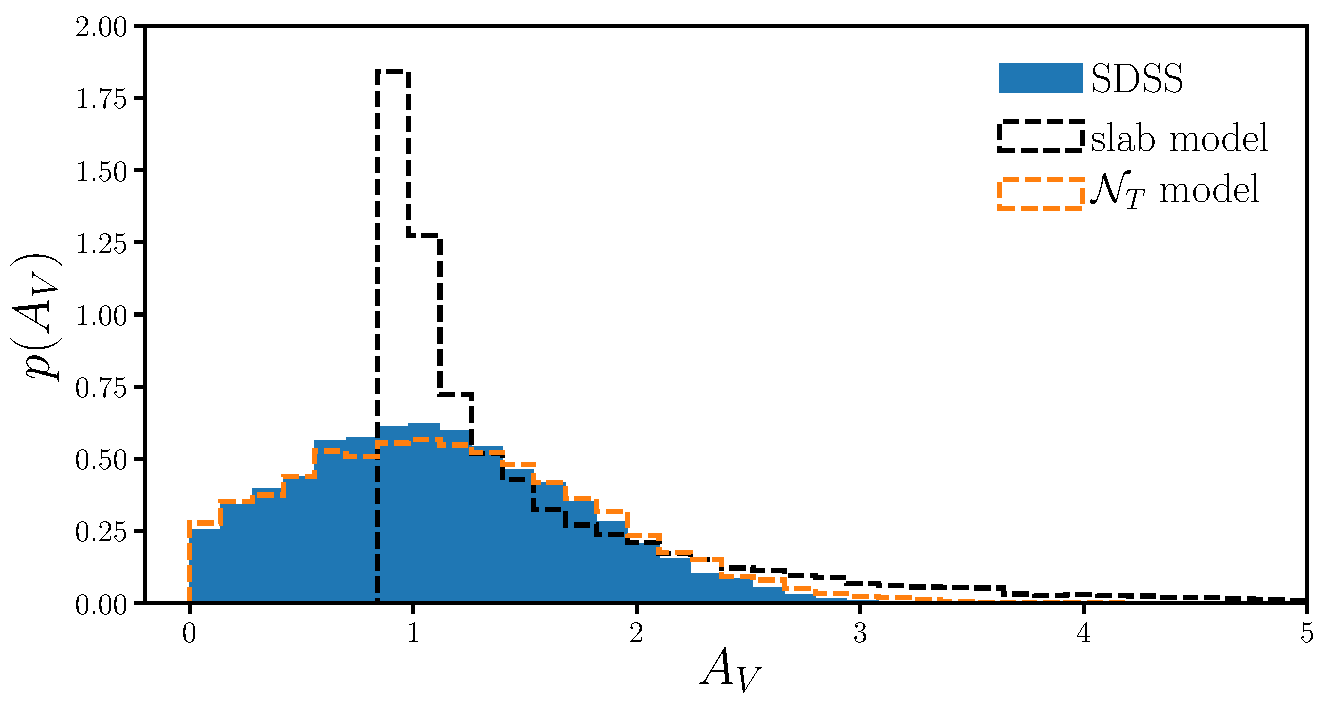
\includegraphics[width=0.66\textwidth]{figs/slab_tnorm.pdf} 
        \caption{Comparison of $A_V$ distribution of SDSS star-forming
        galaxies (blue) to predictions from the slab model (Eq.~\ref{eq:slab};
        black). {\color{red} detail on how SDSS SF galaxies are classified.} 
        The slab model assumes that there's a slab of dust in front of a galaxy.
        We use $\tau_V=2$ for the slab model above. Regardless of $\tau_V$,
        however, the slab model predicts a significantly more asymmetric and peaked $A_V$ distribution
        than observations. Given this disagreement, {\em we include in our
        analysis a DEM with an empirical prescription for $A_V$ based on a truncated normal 
        distribution, which better reproduce the observed $A_V$ distribution} (Section~\ref{sec:nonslab}). }
        \label{fig:av_dist}
    \end{center}
\end{figure}

 
\begin{figure}
    \begin{center}
        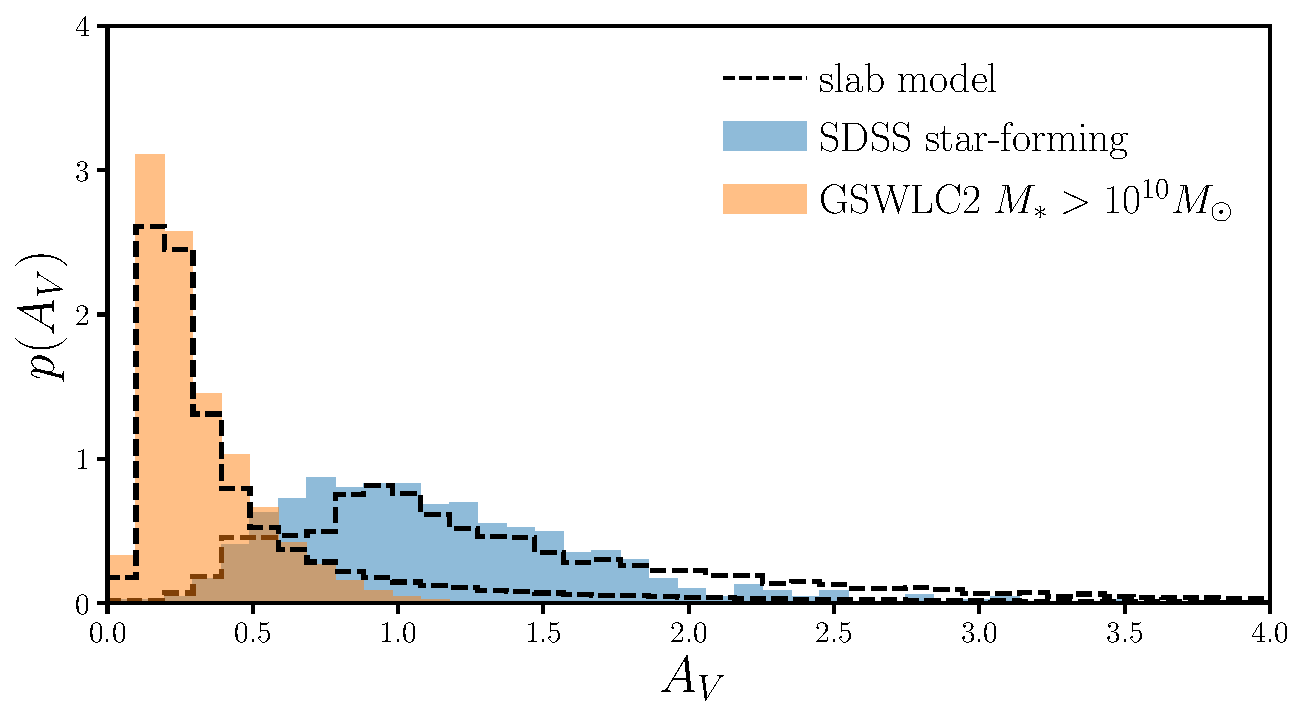
\includegraphics[width=0.66\textwidth]{figs/slab_model.pdf} 
        \caption{\label{fig:av_dist}
        The $A_V$ distributions, $p(A_V)$, generated from the slab model (Eq.~\ref{eq:slab};
        black dash) compared to $p(A_V)$ of star-forming galaxies in SDSS
        (blue) and of $M_* > 10^{10}M_\odot$ galaxies in the \cite{salim2018} GSWLC2 sample (orange). 
        The $A_V$ values for both observations are derived using SED
        fitting~\citep{brinchmann2004, salim2018}. 
        Meanwhile, for the slab model, we generate $A_V$ values for each galaxy
        in the SDSS and GSWLC2 samples using Eq.~\ref{eq:slab} with its
        measured $M_*$ and $\ssfr$. 
        The significant difference between the $p(A_V)$ of SDSS and GSWLC2 is
        due to inconsistencies in the $A_V$ measurements of the two catalogs. 
        It illustrates the challenges in observationally measuring $A_V$ and,
        again, highlights the advantages of our forward modeling approach. 
        Despite the significant differences between the two, the slab model is
        able to generate $p(A_V)$ in good agreement with $p(A_V)$ from both
        observations with parameter values chosen within the
        Table~\ref{tab:free_param} prior range. 
        Therefore, the slab model provides a sufficiently flexible prescription
        for our \eda.
        }
    \end{center}
\end{figure}


\section{The Slab Model Based EDA}  \label{sec:slab} 
\ch{ 
    In our \eda~prescription, we use the slab model to determine $A_V$, the
    amplitude of attenuation, as a function of a randomly sampled inclination,
    $i$, and $\tau_V$ (see Eq.~\ref{eq:slab} in Section~\ref{sec:dem}).
    The slab model is based on the assumption that dust in galaxies have
    slab-like geometry and illuminated by the stellar radiation
    source~\citep{somerville1999}. 
}
For a given $\tau_V$, the attenuation depends solely on the orientation of the galaxy. 
\ch{
    While this simplification reproduces the correlation between $A_V$ and $i$
    found in observed star-forming galaxies~\citep[\eg][]{conroy2010, wild2011,
    battisti2017, salim2020}, it ignores the detailed star-to-dust geometry that
    impacts the attenuation curve. 
    It also does not provide a well-motivated prescription for quiescent
    galaxies, which typically have elliptical morphologies.
    Despite its limitations, the slab model provides a robust empirical
    prescription that allows us to produce realistic distributions of $A_V$. 
}

\ch{ 
    In Figure~\ref{fig:av_dist}, we compare the $A_V$ distributions, $p(A_V)$,
    of star-forming galaxies in SDSS (blue) and galaxies in the
    \cite{salim2018} GSWLC2 sample (orange) to the $p(A_V)$ generated from the
    slab model (black dashed). 
    The $A_V$ values of the SDSS are derived using SED fitting from the
    \cite{brinchmann2004} MPA-JHU catalog.
    The $A_V$ values of the GSWLC2 galaxies are also derived from SED fitting UV and optical
    photometry from GALEX and SDSS observations as well as mid-IR photometry from WISE. 
    We include all GSWLC2 galaxies, including quiescent galaxies, above $M_* > 10^{10}M_\odot$. 
    We generate two $p(A_V)$ with the slab model for the SDSS and GSWLC2
    samples separately.
    For each SDSS/GSWLC2 galaxy, we determine $A_V$ by uniformly sampling 
    $\cos i$ from 0 to 1 and derive $\tau_V$ (Eq.~\ref{eq:tauv}) with the
    galaxy's measured $M_*$ and $\ssfr$. 
    We pick $\mtaum, \mtaus, c_\tau$ values within the prior range
    (Table~\ref{tab:free_param}) by hand to roughly reproduce the SDSS and GSWLC2 $p(A_V)$
    distributions. 
}

\ch{
    Galaxies in SDSS and GSWLC2 have substantially different $p(A_V)$. 
    This is due to inconsistencies in the $A_V$ measurements of MPA-JHU and
    GSWLC2 --- even for the same galaxy, the $A_V$ measurements from the two
    catalogs differ significantly.
    This difference in $p(A_V)$ illustrates the challenges in directly measuring
    dust attenuation and yet again highlights the advantages of our forward
    modeling approach. 
    Despite the dramatic differences between the two, the slab model can
    produce $p(A_V)$ in good agreement with both observed distributions. 
    We therefore conclude that the slab model provides a sufficiently flexible
    prescription to sample a realistic distribution of $A_V$. 
}


\ch{
    In addition to the slab model, in the \eda, we also use a linear
    dependence on $M_*$ and $\ssfr$ in the $V$ band optical depth,
    $\tau_V$ (see Eq.~\ref{eq:tauv}).
    This parameterization is motivated by observations that find significant
    correlation between $A_V$ and $M_*$ and $\ssfr$~\citep[\eg~][]{garn2010, battisti2016, salim2020}. 
    We take a closer look at this correlation using the GWSLC2 sample in
    Figure~\ref{fig:dep}.
    We present the dependence of $A_V$ on $M_*$ (left panel) and $\ssfr$ (right
    panel). 
    In the left panel, we divide the GSWLC2 galaxies by $\ssfr$: 
    $\ssfr < 10^{-11}yr^{-1}$ (purple), $10^{-11} < \ssfr < 10^{-10}yr^{-1}$
    (red), and  $10^{-10} < \ssfr$ (orange). 
    For each of the $\ssfr$ bins, we find significant $\log M_*$ dependence in
    $A_V$: galaxies with higher $\ssfr$ have a stronger $M_*$ dependence.  
    In the right, we divide the galaxies by $M_*$: 
    $10^{9.5} < M_* < 10^{10.5}M_\odot$ (blue) and $10^{10.5} M_\odot < M_*$
    (green).
    Although both $M_*$ bins have some $\ssfr$ dependence, the dependence is
    stronger for galaxies with $M_* > 10^{10.5}M_\odot$. 
    This stellar mass limit roughly corresponds to galaxies that are included
    in our forward model (see Figure~\ref{fig:avmsfr}). 
    The $M_*$ and $\ssfr$ dependence we find in $A_V$ from the GSWLC2 sample is
    consistent with previous observations and further motivates our
    \eda~prescription.
}

\begin{figure}
\begin{center}
    %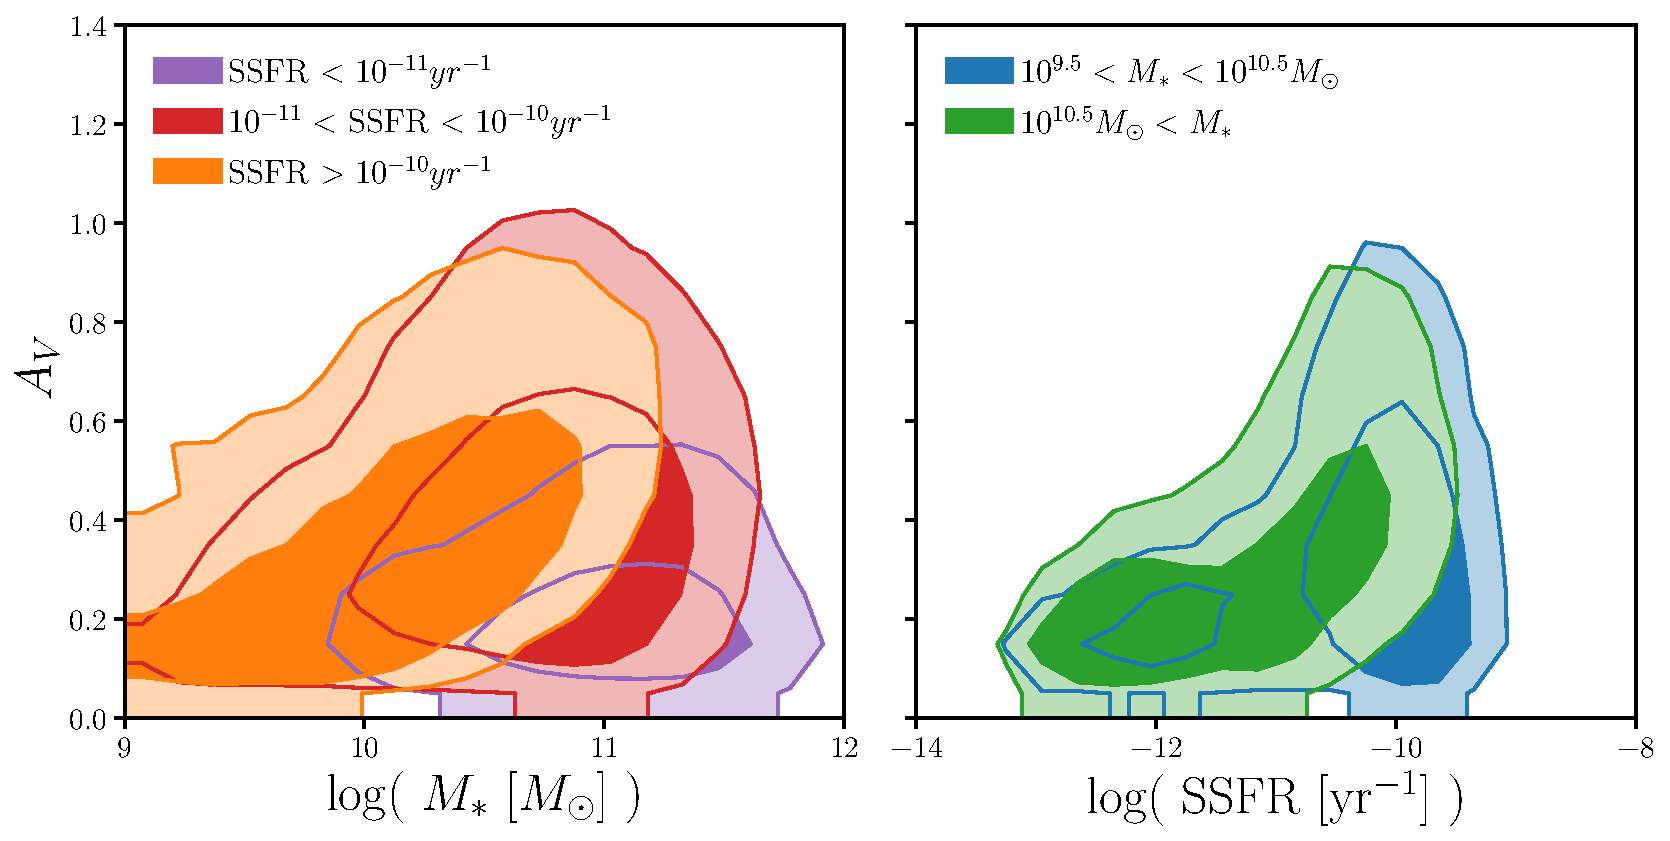
\includegraphics[width=\textwidth]{figs/gswlc_dep.pdf}
    \caption{\label{fig:dep}
    \ch{
        Dependence of $A_V$ on $M_*$ (left) and $\ssfr$ (right) for the
        \cite{salim2018} GSWLC2 sample.
        In the left panel, we divide the GSWLC2 sample into bins of $\ssfr$: 
        $\ssfr < 10^{-11}yr^{-1}$ (purple), 
        $10^{-11} < \ssfr < 10^{-10}yr^{-1}$ (red),
        and  $10^{-10} < \ssfr$ (orange). 
        In each of the $\ssfr$ bins, we find significant $M_*$ dependence. 
        In the right panel, we divide the sample into bins of $M_*$:  
        $10^{9.5} < M_* < 10^{10.5}M_\odot$ (blue) and $10^{10.5} M_\odot < M_*$ (green).
        In the $M_* > 10^{10.5}M_\odot$ bin, which roughly corresponds to our
        SDSS sample, we find significant $\ssfr$ dependence.
        The $M_*$ and $\ssfr$ dependence in $A_V$ we find in GSWLC2 is
        consistent with previous works and provides further motivation for our
        \eda~prescription.
    }
    }
\end{center}
\end{figure}
 

\bibliographystyle{mnras}
\bibliography{galpopfm} 
\end{document}
